\documentclass[11pt,a4paper]{article}
% --- Unicode and language setup for XeLaTeX ---
\usepackage{fontspec}
\usepackage{polyglossia}
\setmainlanguage{greek}
\setotherlanguage{english}
% Choose fonts with good Greek support
\setmainfont{DejaVu Serif}
\setsansfont{DejaVu Sans}
\setmonofont{DejaVu Sans Mono}
% Microtypography
\usepackage{microtype}

% inputenc not needed with XeLaTeX
% babel replaced by polyglossia
\usepackage{amsmath}
\usepackage{amsfonts}
\usepackage{amssymb}
\usepackage{graphicx}
\usepackage{geometry}
\usepackage[unicode]{hyperref}
\usepackage{listings}
\usepackage{xcolor}
\usepackage{float}
\usepackage{caption}
\usepackage{subcaption}
\usepackage{booktabs}
\usepackage{array}

\geometry{margin=2.5cm}

% Code styling
\lstset{
    basicstyle=\ttfamily\footnotesize,
    breaklines=true,
    frame=single,
    numbers=left,
    numberstyle=\tiny,
    keywordstyle=\color{blue}
% Unicode-friendly settings for listings
\lstset{columns=fullflexible, upquote=true, keepspaces=true}
,
    commentstyle=\color{green},
    stringstyle=\color{red}
}

\title{\textbf{Διαδραστική Εφαρμογή Streamlit για\\Ανάλυση Single-Cell RNA Sequencing:\\Ολοκληρωμένη Πλατφόρμα Μοριακής Βιολογίας}}

\author{
    Ομάδα Μοριακής Βιολογίας\\
    \texttt{GitHub: https://github.com/your-repo/molecular-biology-app}
}

\date{\today}

\begin{document}

\maketitle

\begin{abstract}
Αυτή η εργασία παρουσιάζει τον σχεδιασμό, την υλοποίηση και την ανάπτυξη μιας ολοκληρωμένης διαδικτυακής εφαρμογής για ανάλυση δεδομένων single-cell RNA sequencing (scRNA-seq). Η εφαρμογή, που αναπτύχθηκε με το framework Streamlit, παρέχει μια ενοποιημένη πλατφόρμα για προεπεξεργασία δεδομένων, έλεγχο ποιότητας, ενοποίηση, ανάλυση διαφορικής γονιδιακής έκφρασης, μείωση διαστάσεων, οπτικοποίηση και σχολιασμό τύπων κυττάρων. Το σύστημα ενσωματώνει προηγμένες τεχνικές διαχείρισης μνήμης, έτοιμο για παραγωγή χειρισμό σφαλμάτων και βελτιστοποιήσεις επιστημονικού υπολογισμού για αποδοτικό χειρισμό μεγάλων γονιδιωματικών δεδομένων. Η εφαρμογή είναι πλήρως containerized με Docker για απρόσκοπτη ανάπτυξη σε διαφορετικά περιβάλλοντα. Βασικές καινοτομίες περιλαμβάνουν προσαρμοστική διαχείριση μνήμης, παρακολούθηση απόδοσης σε πραγματικό χρόνο και μια modular αρχιτεκτονική που εξασφαλίζει τόσο επιστημονική ακρίβεια όσο και υπολογιστική αποδοτικότητα.

\textbf{Λέξεις-κλειδιά:} Single-cell RNA sequencing, Streamlit, Βιοπληροφορική, Ανάλυση Δεδομένων, Docker, Διαχείριση Μνήμης, Επιστημονικός Υπολογισμός
\end{abstract}

\section{Εισαγωγή}

Η τεχνολογία Single-cell RNA sequencing (scRNA-seq) έχει επαναστατήσει την κατανόησή μας για την κυτταρική ετερογένεια και τη δυναμική της γονιδιακής έκφρασης σε επίπεδο μεμονωμένου κυττάρου. Η ανάλυση δεδομένων scRNA-seq απαιτεί εξελιγμένα υπολογιστικά pipelines που μπορούν να χειριστούν μεγάλα σύνολα δεδομένων διατηρώντας παράλληλα την επιστημονική ακρίβεια και παρέχοντας διαισθητικές διεπαφές χρήστη για τους ερευνητές.

Αυτή η εργασία παρουσιάζει μια ολοκληρωμένη διαδικτυακή πλατφόρμα που αναπτύχθηκε ειδικά για ανάλυση δεδομένων scRNA-seq, αντιμετωπίζοντας κρίσιμες προκλήσεις στη βιοπληροφορική:

\begin{itemize}
    \item \textbf{Κλιμακωσιμότητα}: Χειρισμός δεδομένων με εκατομμύρια κύτταρα και δεκάδες χιλιάδες γονίδια
    \item \textbf{Αποδοτικότητα Μνήμης}: Προηγμένη διαχείριση μνήμης για περιβάλλοντα με περιορισμένους πόρους
    \item \textbf{Επιστημονική Ακρίβεια}: Διατήρηση στατιστικής αυστηρότητας χωρίς συμβιβασμούς στην απόδοση
    \item \textbf{Εμπειρία Χρήστη}: Διαισθητική διεπαφή για ερευνητές χωρίς εκτεταμένη γνώση προγραμματισμού
    \item \textbf{Αναπαραγωγιμότητα}: Containerized ανάπτυξη που εξασφαλίζει συνεπή αποτελέσματα σε όλες τις πλατφόρμες
\end{itemize}

Η εφαρμογή ενσωματώνει αλγορίθμους αιχμής από το οικοσύστημα Scanpy με προσαρμοσμένες βελτιστοποιήσεις για ανάπτυξη έτοιμη για παραγωγή.

\section{Σχεδιασμός της Υλοποίησης}

\subsection{Αρχιτεκτονική Συστήματος}

Η εφαρμογή ακολουθεί ένα μοντέλο modular αρχιτεκτονικής, διαχωρίζοντας τις αρμοδιότητες σε διαφορετικές λειτουργικές ενότητες:

\begin{itemize}
    \item \textbf{Ενότητα Προεπεξεργασίας Δεδομένων}: Έλεγχος ποιότητας, φιλτράρισμα, κανονικοποίηση
    \item \textbf{Ενότητα Ενοποίησης Δεδομένων}: Ενοποίηση πολλαπλών datasets με Scanorama και μεθόδους concatenation
    \item \textbf{Ενότητα Διαφορικής Έκφρασης}: Στατιστική ανάλυση με διόρθωση πολλαπλών δοκιμών
    \item \textbf{Ενότητα Οπτικοποίησης}: Διαδραστικά γραφήματα με Plotly και Matplotlib
    \item \textbf{Ενότητα Σχολιασμού Κυττάρων}: Αυτοματοποιημένη και χειροκίνητη αναγνώριση τύπων κυττάρων
    \item \textbf{Εργαλεία Διαχείρισης Μνήμης}: Προηγμένη παρακολούθηση και βελτιστοποίηση μνήμης
\end{itemize}

\subsection{Στοίβα Τεχνολογιών}

\begin{table}[H]
\centering
\caption{Συστατικά Στοίβας Τεχνολογιών}
\begin{tabular}{@{}ll@{}}
\toprule
\textbf{Κατηγορία} & \textbf{Τεχνολογίες} \\
\midrule
Frontend Framework & Streamlit 1.28+ \\
Επιστημονικός Υπολογισμός & NumPy, SciPy, Pandas \\
Βιοπληροφορική & Scanpy, AnnData, Scanorama \\
Οπτικοποίηση & Plotly, Matplotlib, Seaborn \\
Στατιστική Ανάλυση & Statsmodels, Scikit-learn \\
Διαχείριση Μνήμης & psutil, προσαρμοσμένος AdvancedMemoryManager \\
Containerization & Docker, Docker Compose \\
\bottomrule
\end{tabular}
\end{table}

\subsection{Πρότυπα Σχεδίασης}

Η υλοποίηση ενσωματώνει διάφορα πρότυπα σχεδίασης:

\begin{itemize}
    \item \textbf{Module Pattern}: Κάθε τύπος ανάλυσης είναι ενθυλακωμένος στη δική του ενότητα
    \item \textbf{Singleton Pattern}: Ο διαχειριστής μνήμης εξασφαλίζει ένα μόνο στιγμιότυπο σε όλη την εφαρμογή
    \item \textbf{Observer Pattern}: Παρακολούθηση μνήμης σε πραγματικό χρόνο και ειδοποιήσεις
\begin{figure}
        \centering
        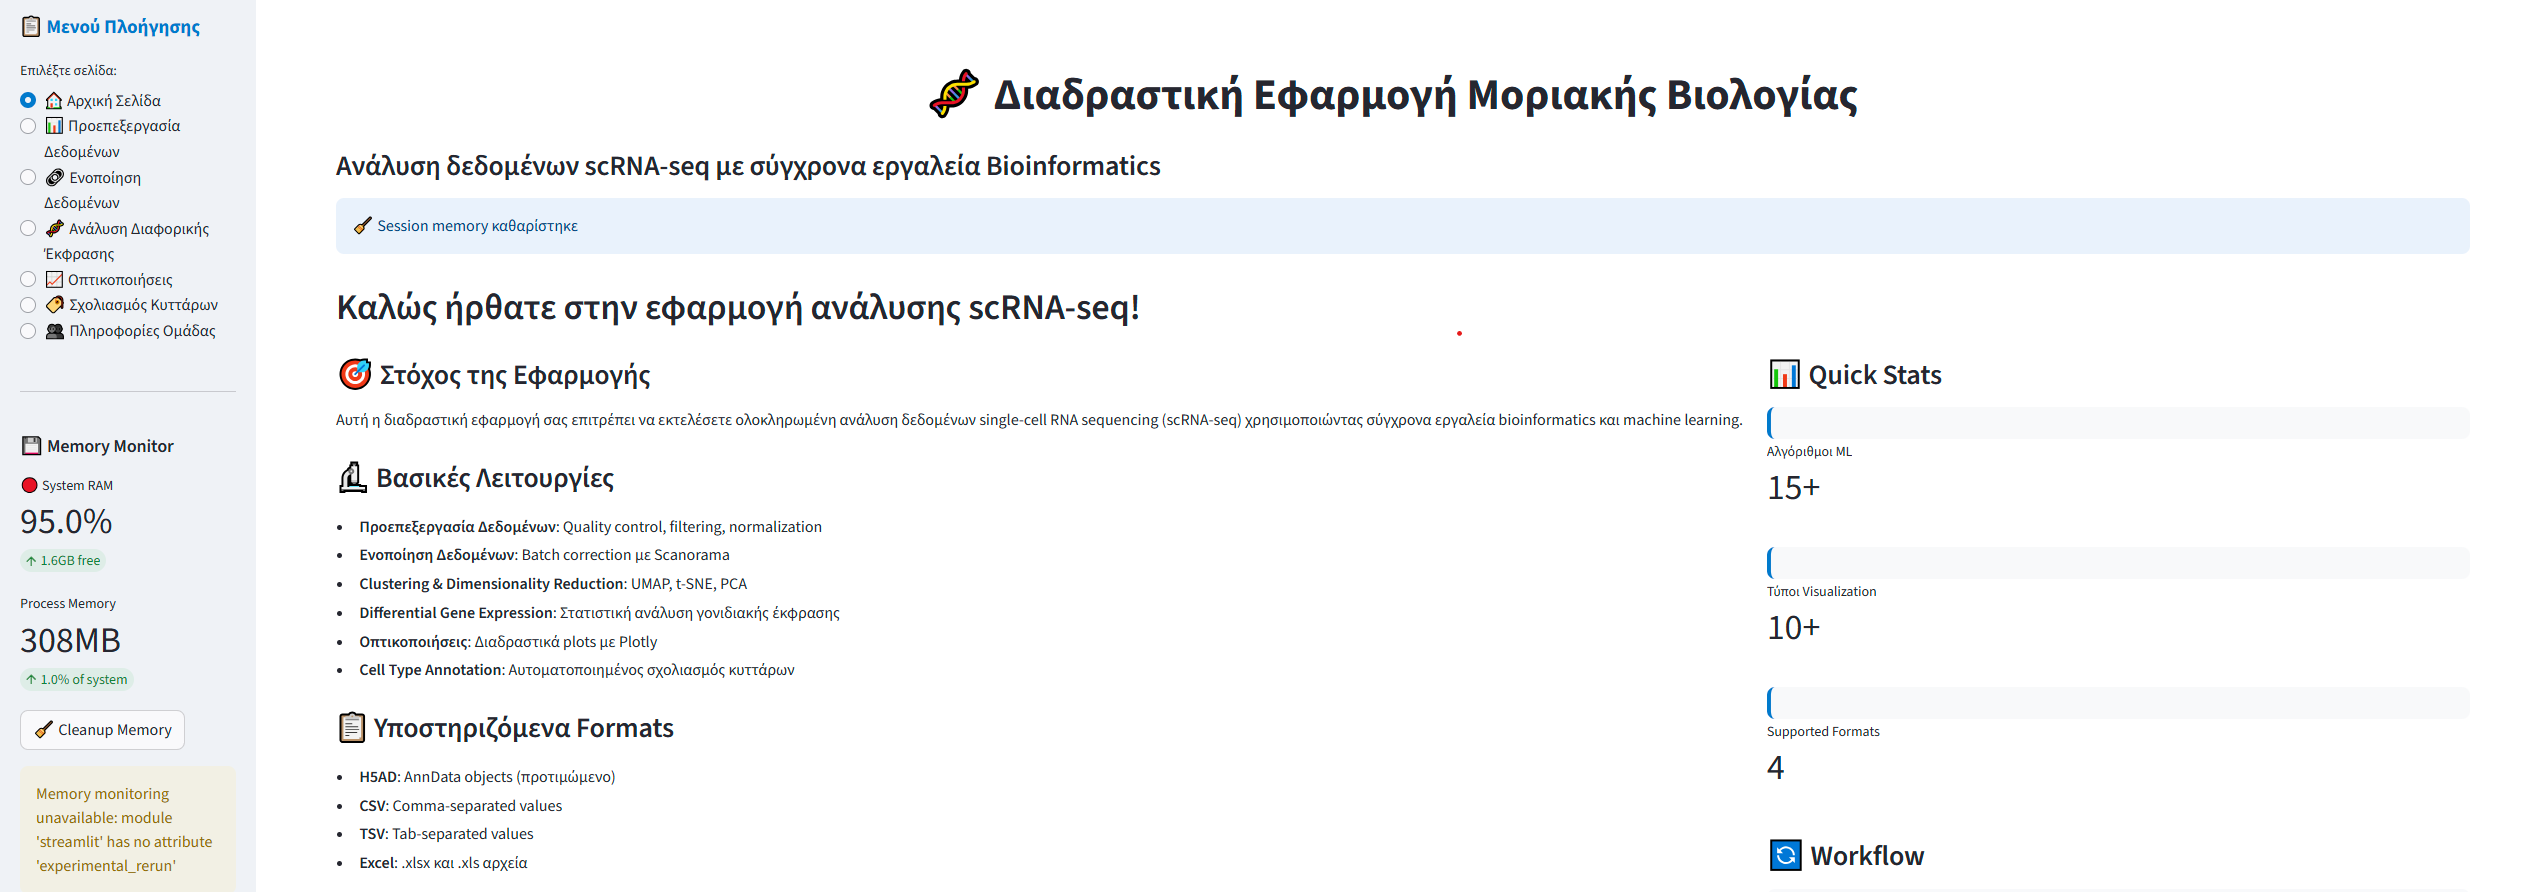
\includegraphics[scale=0.5]{main.png}
        \caption{Κύρια Εφαρμογή}
        \label{fig:placeholder}
    \end{figure}
        \item \textbf{Strategy Pattern}: Πολλαπλές μέθοδοι ενοποίησης και ανάλυσης
\end{itemize}




\section{UML Διαγράμματα}

\subsection{Διάγραμμα Κλάσεων}

Το διάγραμμα κλάσεων απεικονίζει τις σχέσεις μεταξύ των κύριων συστατικών του συστήματος:

\begin{figure}
    \centering
    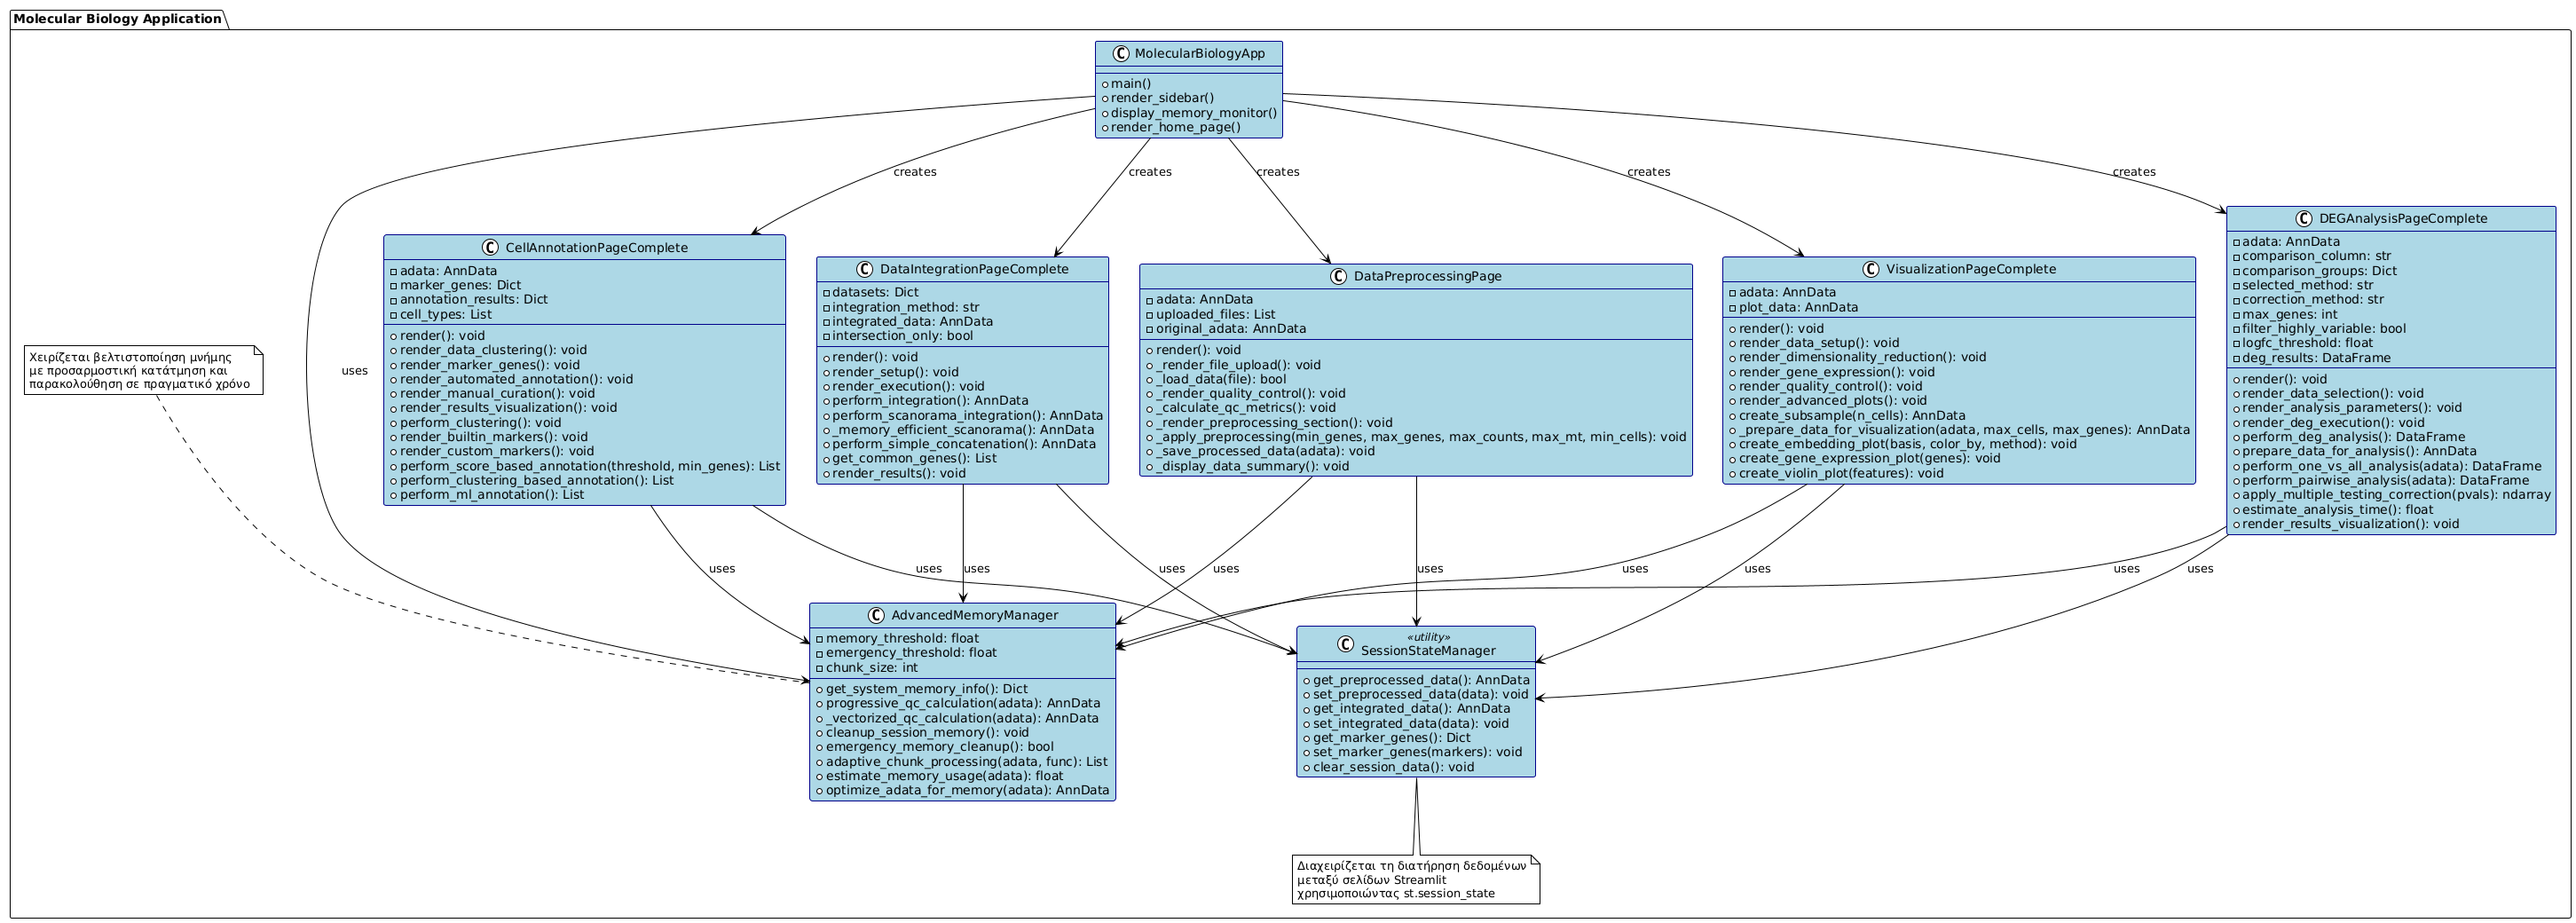
\includegraphics[width=1.0\linewidth]{UML_Class_Diagram.png}
    \caption{Class Diagram}
    \label{fig:placeholder}
\end{figure}

Βασικές κλάσεις περιλαμβάνουν:
\begin{itemize}
    \item \textbf{MolecularBiologyApp}: Κύριος ελεγκτής εφαρμογής
    \item \textbf{AdvancedMemoryManager}: Βελτιστοποίηση και παρακολούθηση μνήμης
    \item \textbf{DataPreprocessingPage}: Έλεγχος ποιότητας και προεπεξεργασία
    \item \textbf{DEGAnalysisPageComplete}: Ανάλυση διαφορικής έκφρασης
    \item \textbf{CellAnnotationPageComplete}: Σχολιασμός τύπων κυττάρων
    \item \textbf{SessionStateManager}: Διατήρηση δεδομένων μεταξύ σελίδων
\end{itemize}

\subsection{Διάγραμμα Περιπτώσεων Χρήσης}

Το διάγραμμα περιπτώσεων χρήσης καταδεικνύει τις λειτουργικές απαιτήσεις και τις αλληλεπιδράσεις χρήστη:

\begin{figure}[H]
    \centering
    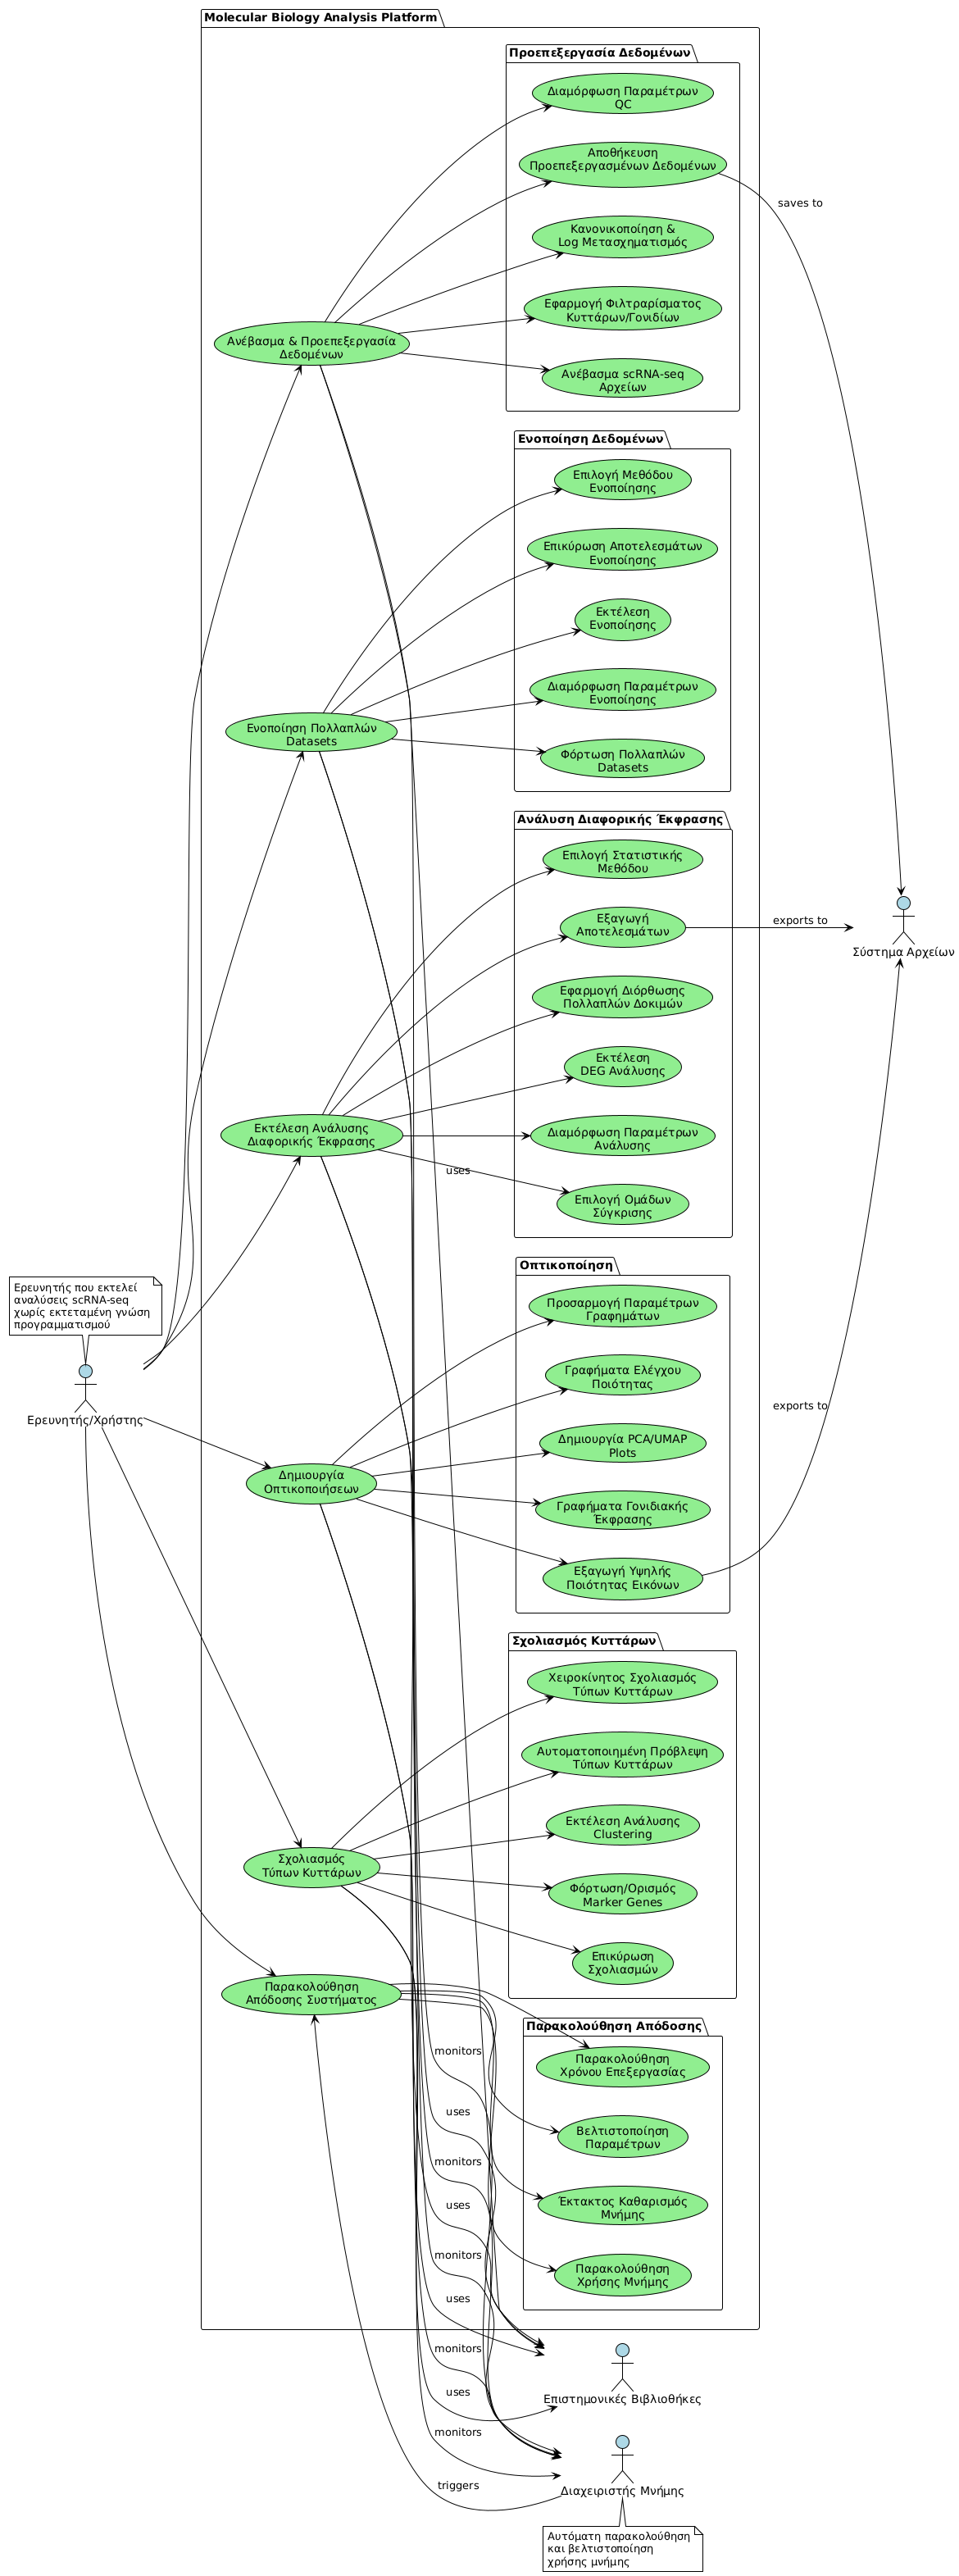
\includegraphics[width=0.5\linewidth]{UML_UseCase_Diagram.png}
    \caption{UML Διάγραμμα Περιπτώσεων Χρήσης που δείχνει τις αλληλεπιδράσεις χρήστη και τη λειτουργικότητα συστήματος}
    \label{fig:use_case_diagram}
\end{figure}

\begin{figure}[H]
    \centering
    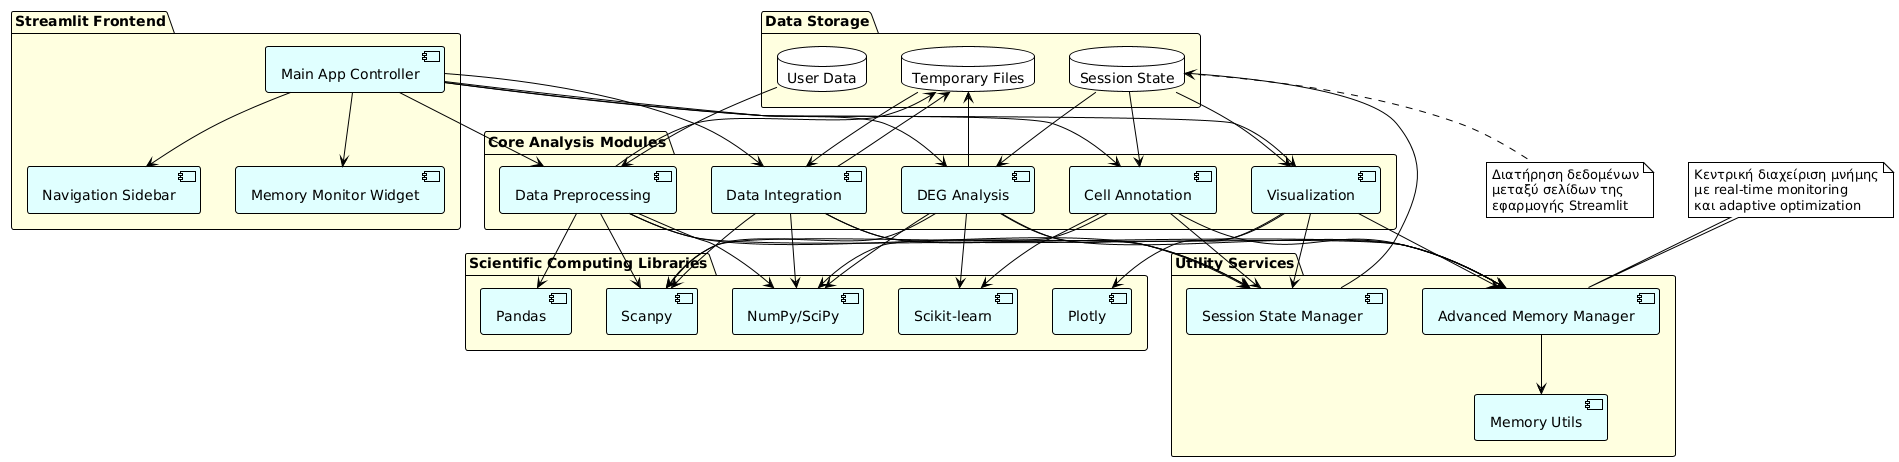
\includegraphics[width=1.0\linewidth]{UML_Component_Diagram.png}
    \caption{UML Component Diagram}
    \label{fig:component_diagram}
\end{figure}
\section{Ανάλυση της Υλοποίησης της Εφαρμογής}

\subsection{Προηγμένη Διαχείριση Μνήμης}

Μια από τις πιο κρίσιμες καινοτομίες σε αυτή την υλοποίηση είναι η κλάση \texttt{AdvancedMemoryManager}, σχεδιασμένη για να χειρίζεται αποδοτικά μεγάλα γονιδιωματικά datasets:

\begin{lstlisting}[language=Python, caption={Υλοποίηση Προηγμένης Διαχείρισης Μνήμης}]
class AdvancedMemoryManager:
    def __init__(self, memory_threshold=0.85, emergency_threshold=0.95):
        self.memory_threshold = memory_threshold
        self.emergency_threshold = emergency_threshold
    
    def progressive_qc_calculation(self, adata):
        """Προσαρμοστική κατάτμηση για υπολογισμό QC μετρικών"""
        memory_info = self.get_system_memory_info()
        
        # Προσαρμοστικό μέγεθος chunk βάσει διαθέσιμης μνήμης
        if memory_info['available_gb'] < 2:
            chunk_size = max(1000, int(adata.n_obs / 20))
        elif memory_info['available_gb'] < 4:
            chunk_size = max(2000, int(adata.n_obs / 10))
        else:
            chunk_size = max(10000, int(adata.n_obs / 3))
        
        return self._process_chunks(adata, chunk_size)
\end{lstlisting}

\subsection{Pipeline Επεξεργασίας Δεδομένων}

Το pipeline επεξεργασίας δεδομένων υλοποιεί μια ισχυρή ροή εργασίας:

\begin{enumerate}
    \item \textbf{Φόρτωση Δεδομένων}: Υποστήριξη για H5AD, CSV και Excel μορφές
    \item \textbf{Έλεγχος Ποιότητας}: Αυτοματοποιημένος υπολογισμός QC μετρικών (n\_genes, total\_counts, μιτοχονδριακό ποσοστό)
    \item \textbf{Φιλτράρισμα}: Φιλτράρισμα κυττάρων και γονιδίων με επικύρωση για αποφυγή κενών datasets
    \item \textbf{Κανονικοποίηση}: Log1p μετασχηματισμός με κατάλληλο χειρισμό σφαλμάτων
    \item \textbf{Διαχείριση Συνεδρίας}: Διατηρητική αποθήκευση σε όλες τις σελίδες της εφαρμογής
\end{enumerate}

\subsection{Υλοποίηση Στατιστικής Ανάλυσης}

Η ενότητα ανάλυσης διαφορικής έκφρασης υλοποιεί πολλαπλές στατιστικές μεθόδους:

\begin{itemize}
    \item \textbf{Wilcoxon Rank-Sum Test}: Μη-παραμετρική μέθοδος για ισχυρές συγκρίσεις
    \item \textbf{T-test}: Παραμετρική μέθοδος για κανονικά κατανεμημένα δεδομένα
    \item \textbf{Logistic Regression}: Για σενάρια δυαδικής κατηγοριοποίησης
    \item \textbf{Διόρθωση Πολλαπλών Δοκιμών}: FDR και Bonferroni μέθοδοι
\end{itemize}

\subsection{Χειρισμός Σφαλμάτων και Επικύρωση}

Ολοκληρωμένος χειρισμός σφαλμάτων εξασφαλίζει τη σταθερότητα της εφαρμογής:

\begin{lstlisting}[language=Python, caption={Παράδειγμα Ισχυρού Χειρισμού Σφαλμάτων}]
def _apply_preprocessing(self, min_genes, max_genes, max_counts, max_mt, min_cells):
    try:
        # Επικύρωση πριν το φιλτράρισμα
        cells_passing = cell_filter.sum()
        if cells_passing == 0:
            st.error("ΚΡΙΣΙΜΟ: Όλα τα κύτταρα θα φιλτραριστούν!")
            st.error("Χαλαρώστε τις παραμέτρους φιλτραρίσματος!")
            return
        
        # Εφαρμογή φιλτραρίσματος με επικύρωση
        self.adata = self.adata[cell_filter, :]
        
    except Exception as e:
        st.error(f"Σφάλμα προεπεξεργασίας: {str(e)}")
        st.info("Παρακαλώ ελέγξτε τις παραμέτρους σας και δοκιμάστε ξανά")
\end{lstlisting}

\section{Οπτικοποιήσεις των Αποτελεσμάτων}

Η εφαρμογή παρέχει ολοκληρωμένες δυνατότητες οπτικοποίησης:

\subsection{Γραφήματα Μείωσης Διαστάσεων}

\begin{figure}[H]
    \centering
    \begin{subfigure}{0.45\textwidth}
       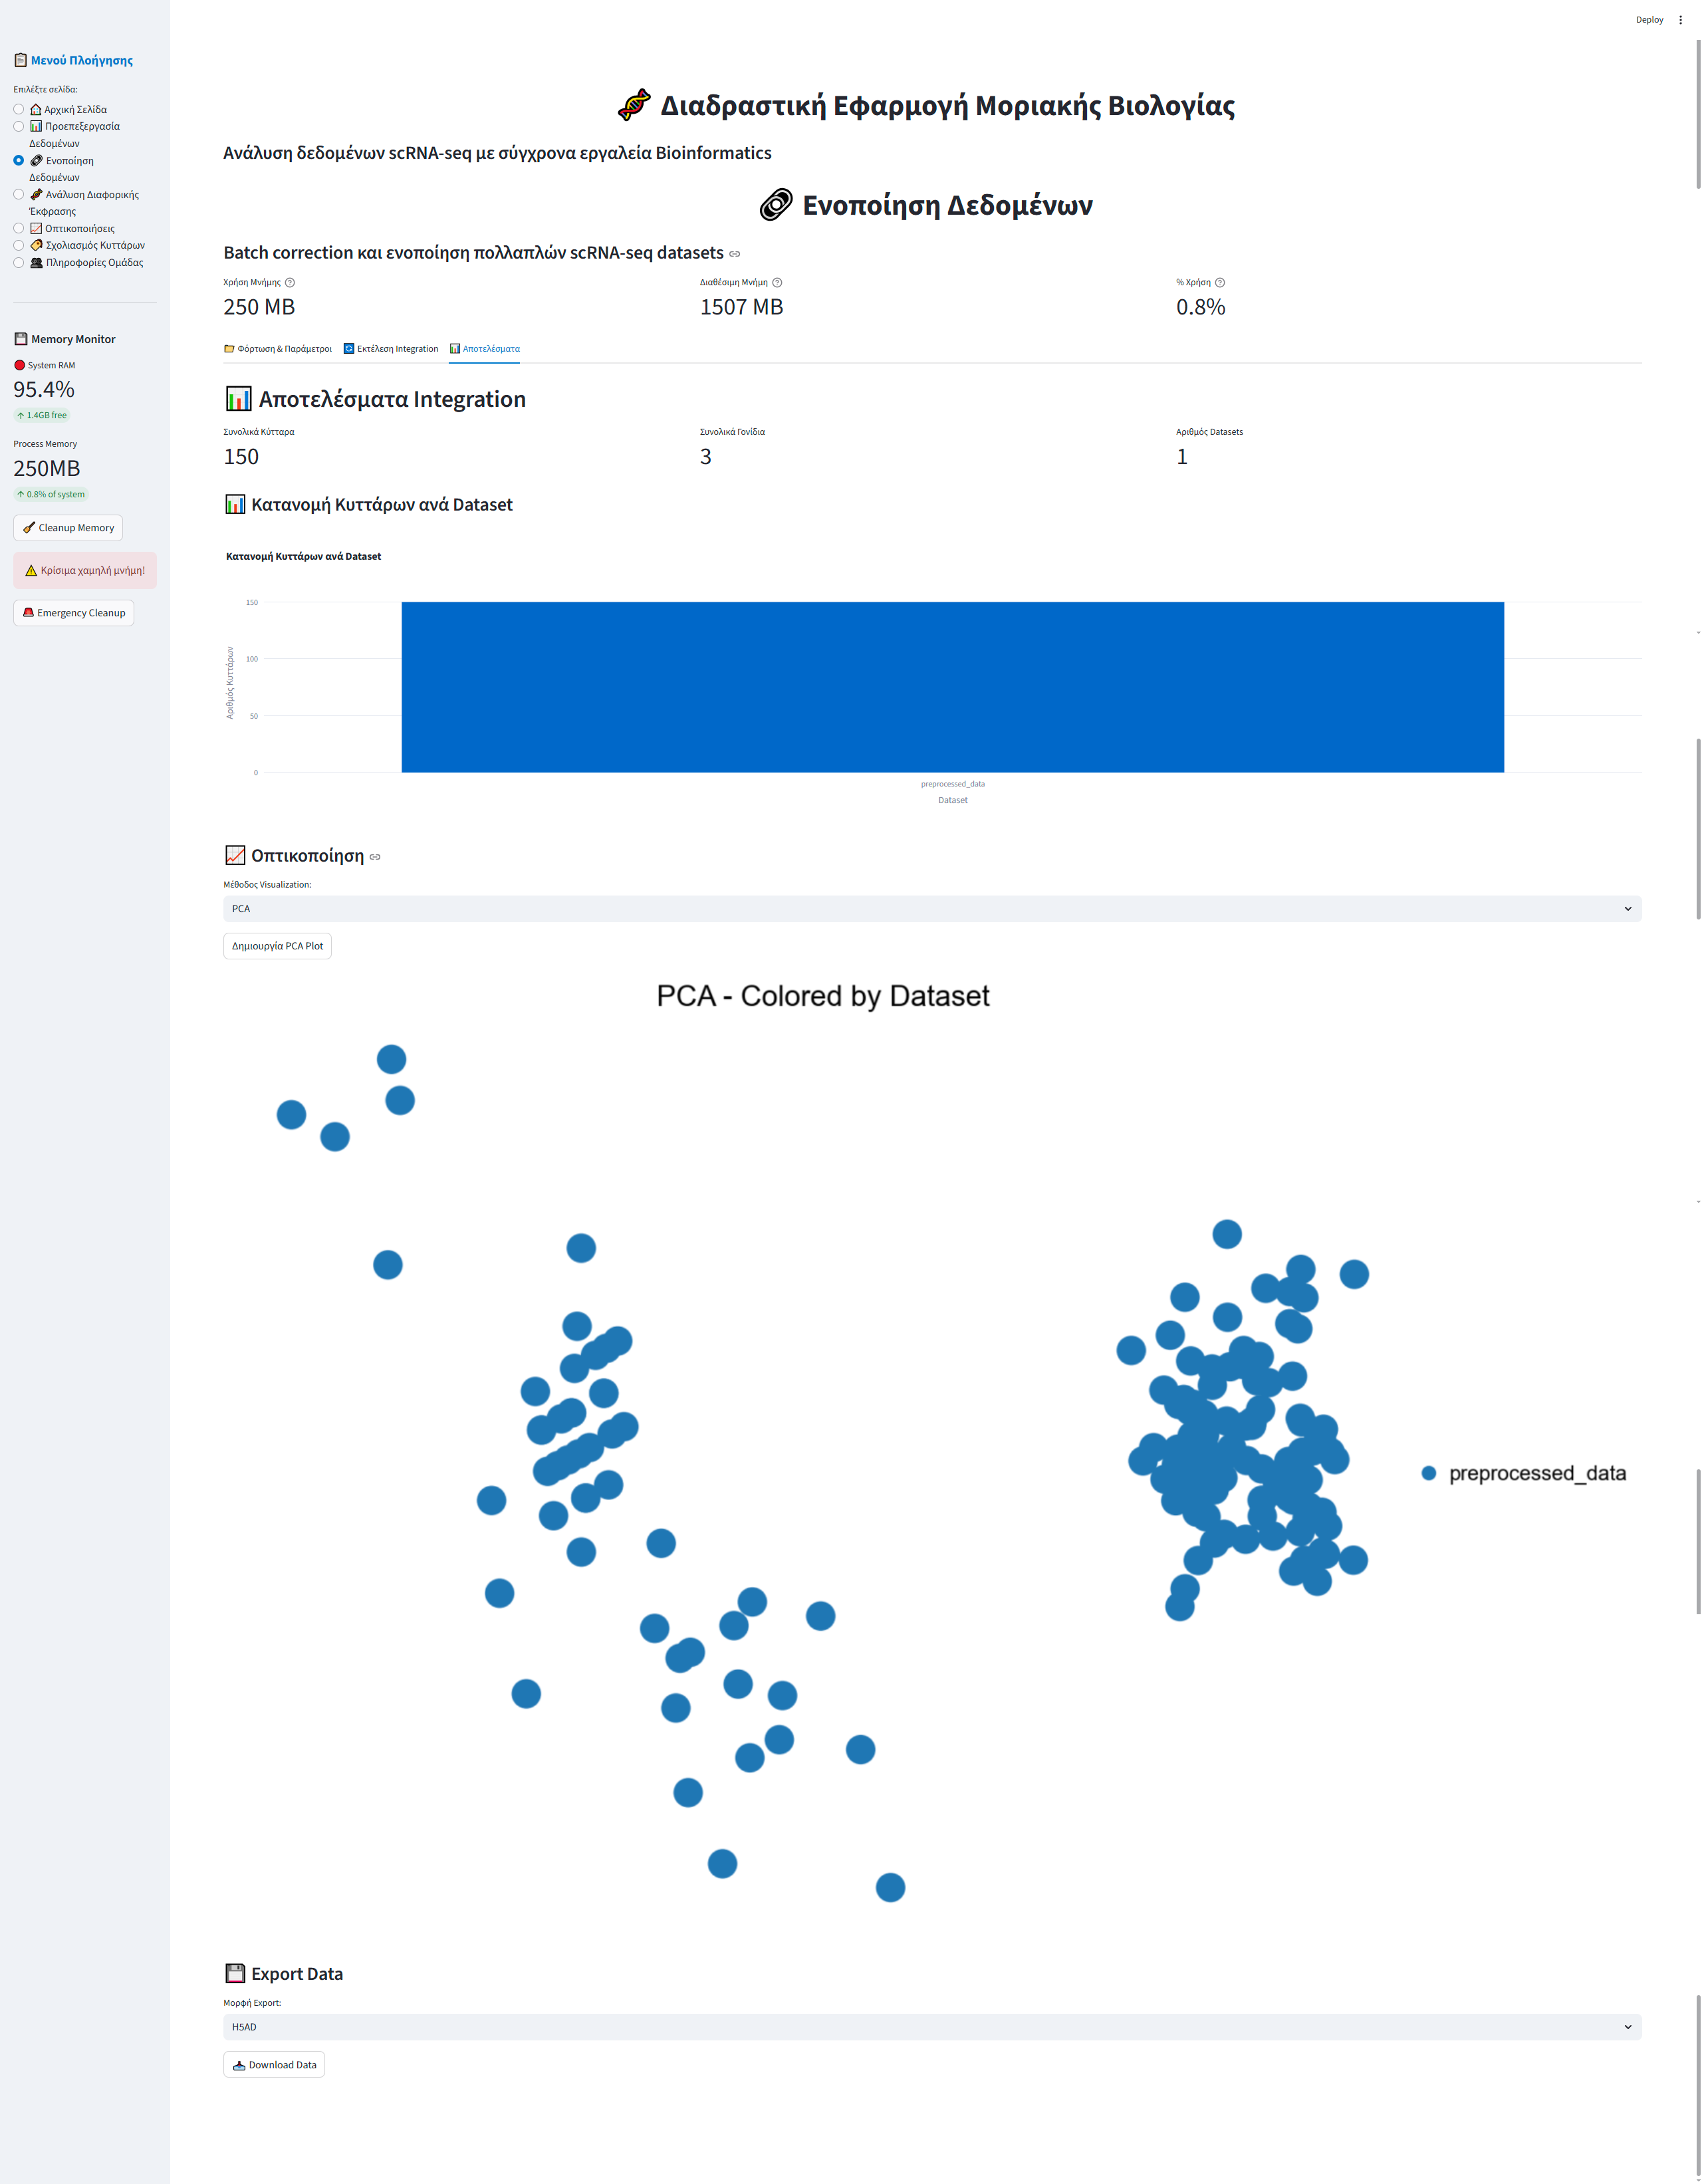
\includegraphics[width=1.0\linewidth]{pca_plot.png}
        \caption{Ανάλυση PCA}
    \end{subfigure}
    \hfill
    \begin{subfigure}{0.45\textwidth}
         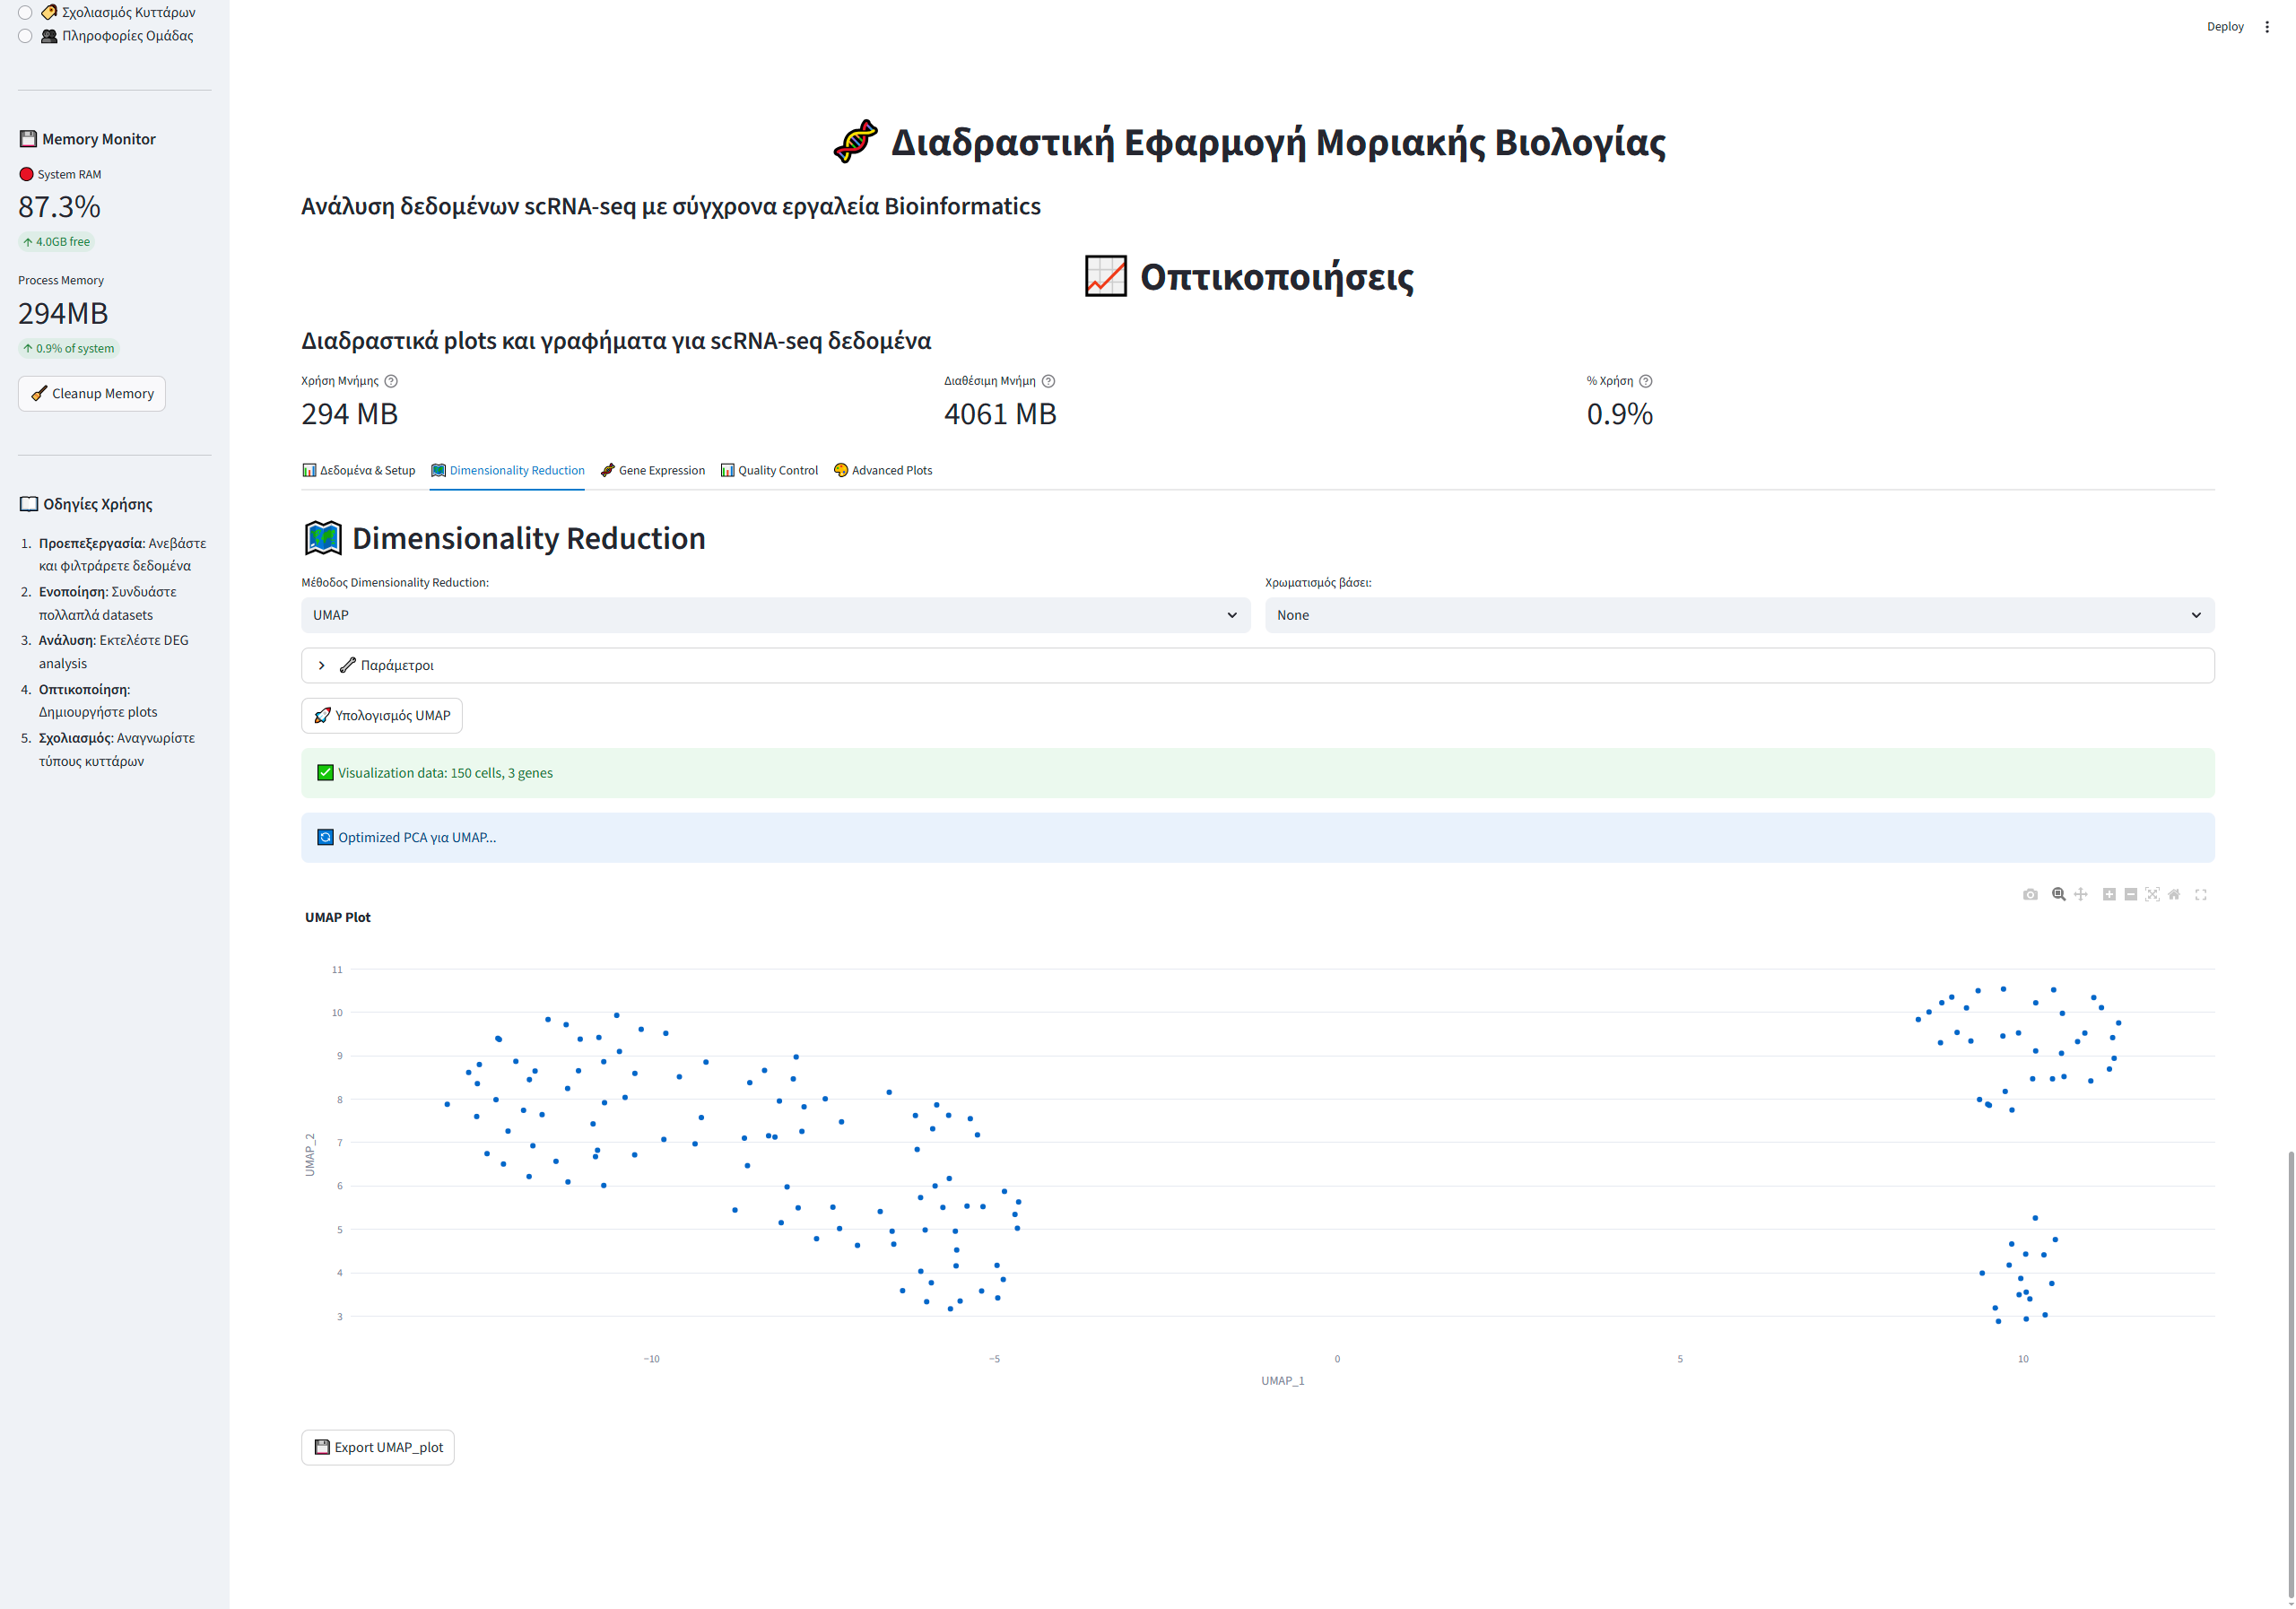
\includegraphics[width=1.0\linewidth]{umap.png}
        \caption{Οπτικοποίηση UMAP}
    \end{subfigure}
    \caption{Οπτικοποιήσεις μείωσης διαστάσεων που δείχνουν μοτίβα ομαδοποίησης κυττάρων}
    \label{fig:dimred}
\end{figure}

\subsection{Μετρικές Ελέγχου Ποιότητας}

\begin{figure}[H]
    \centering
   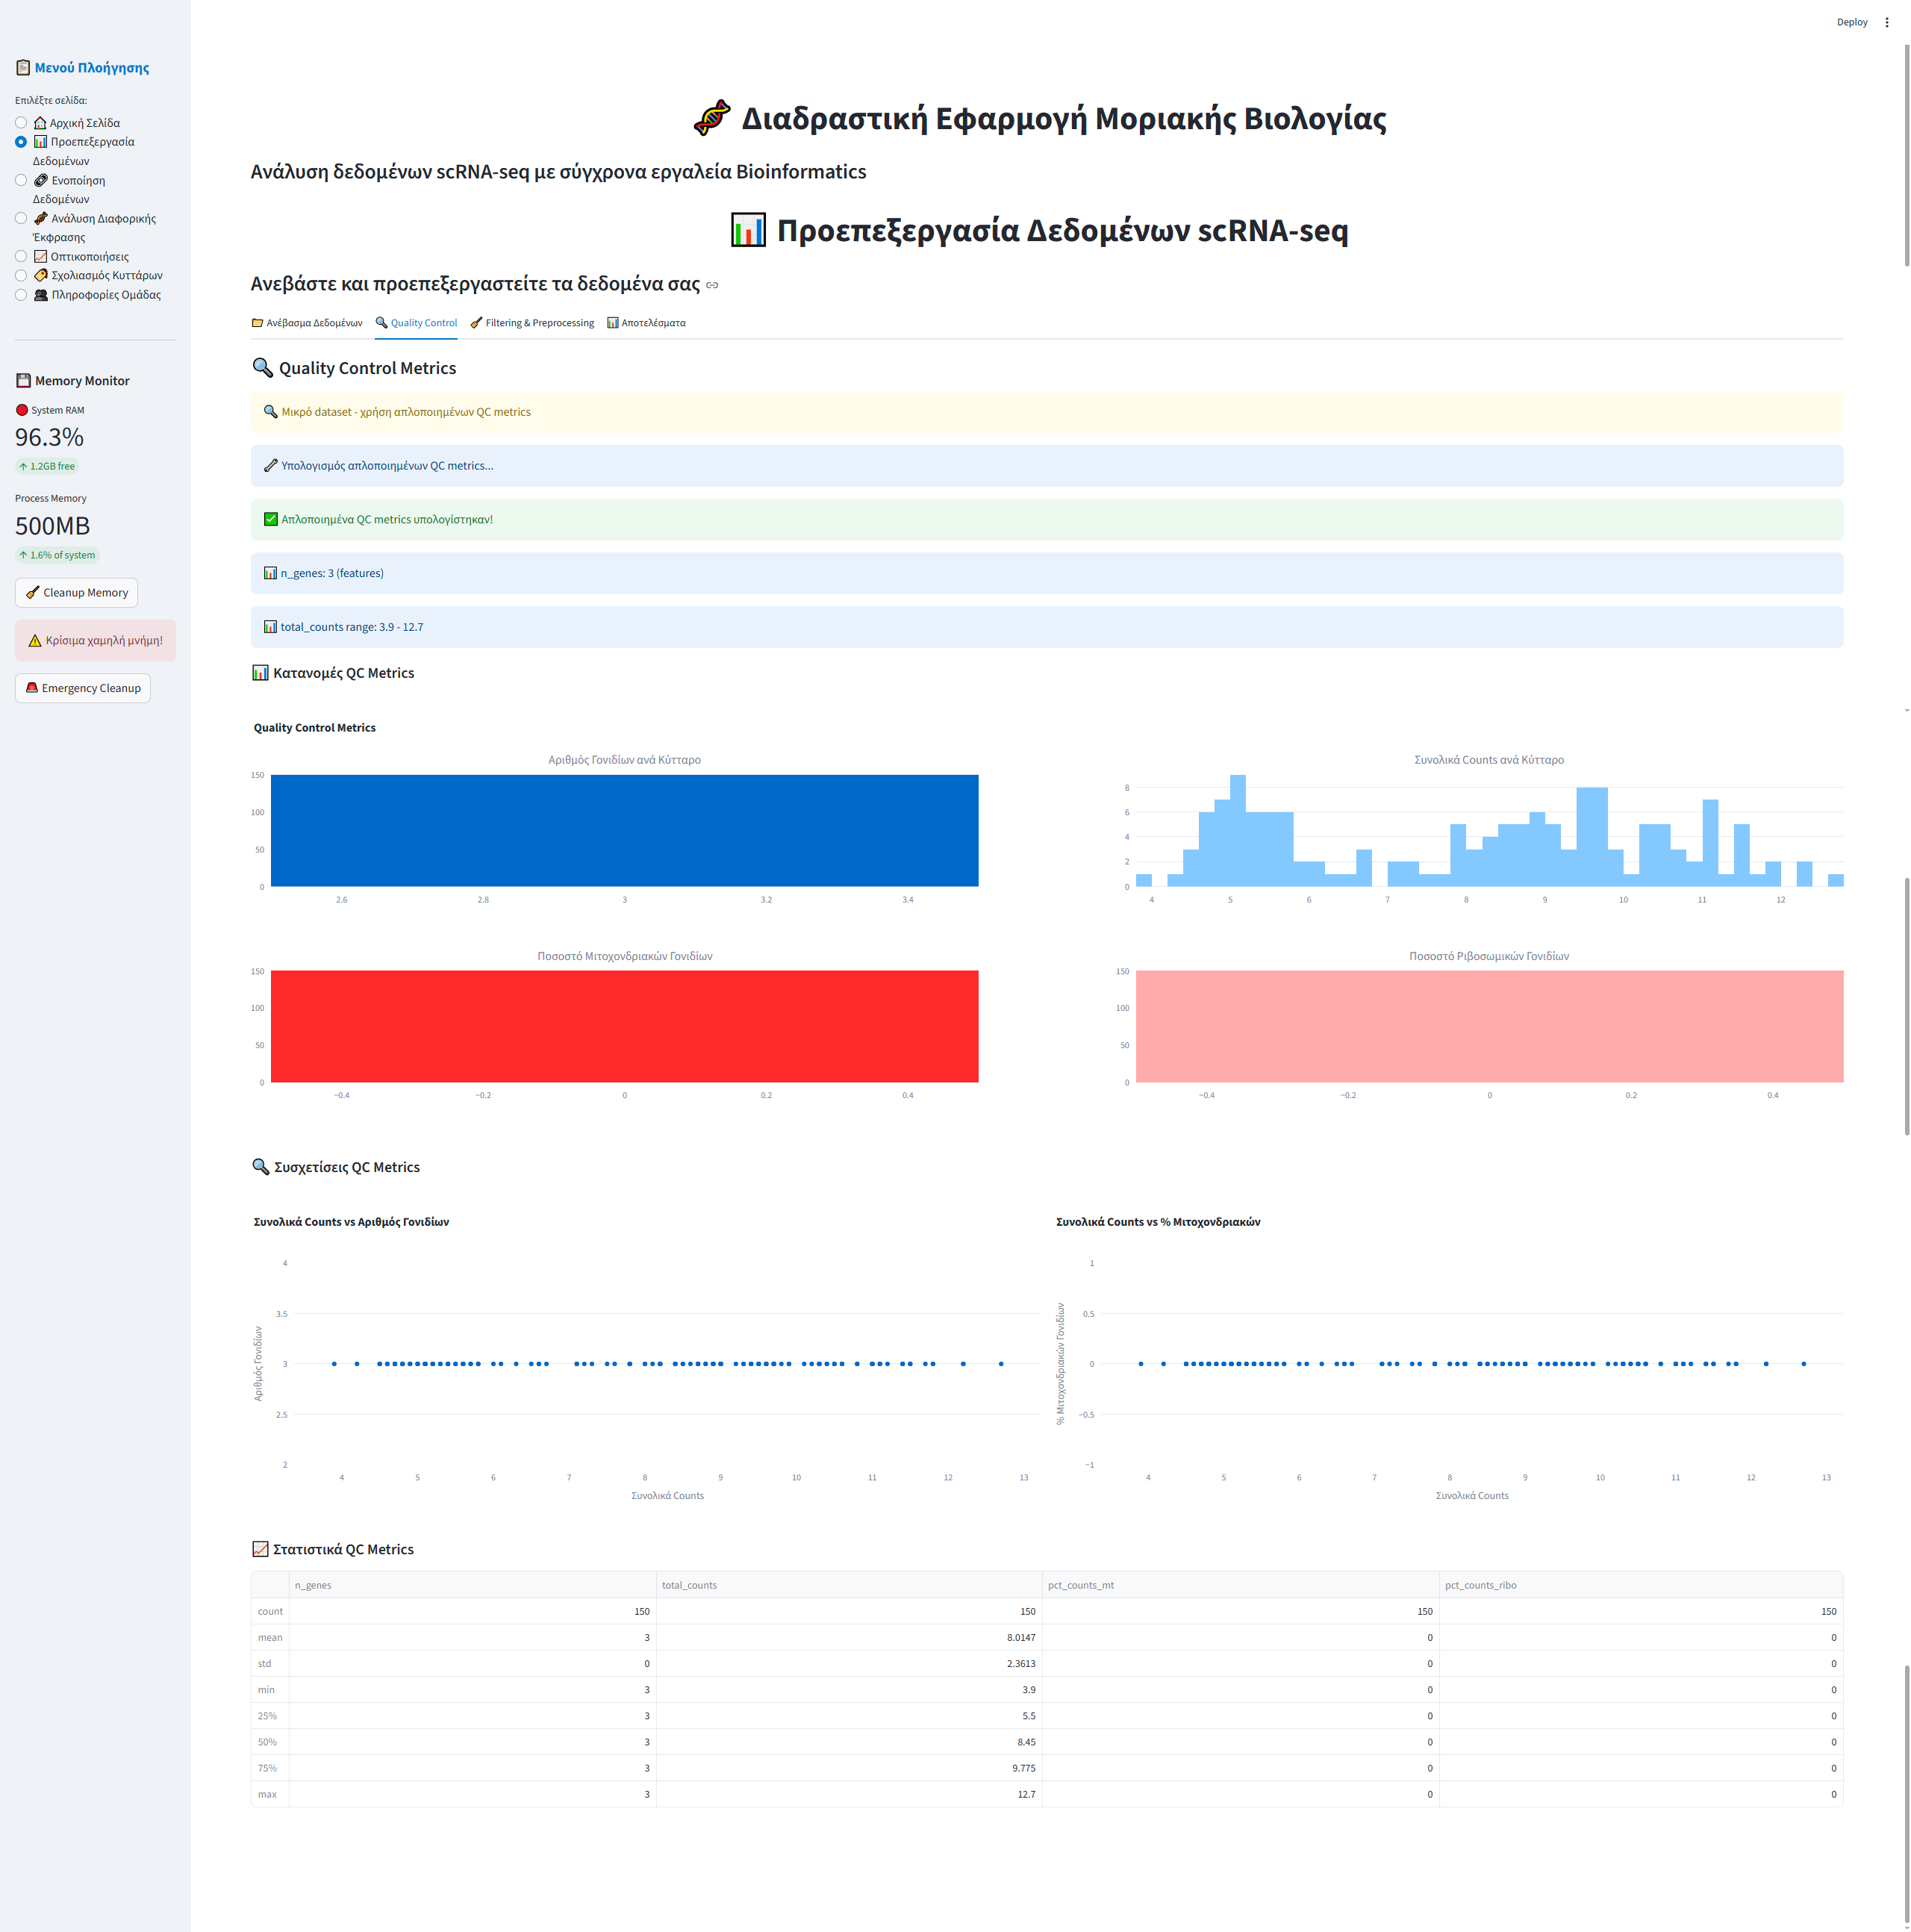
\includegraphics[width=1.0\linewidth]{qc_metrics.png}
    \caption{Οπτικοποίηση μετρικών ελέγχου ποιότητας}
    \label{fig:qc_metrics}
\end{figure}

\subsection{Αποτελέσματα Διαφορικής Έκφρασης}

\begin{figure}[H]
    \centering
    \begin{subfigure}{0.45\textwidth}
         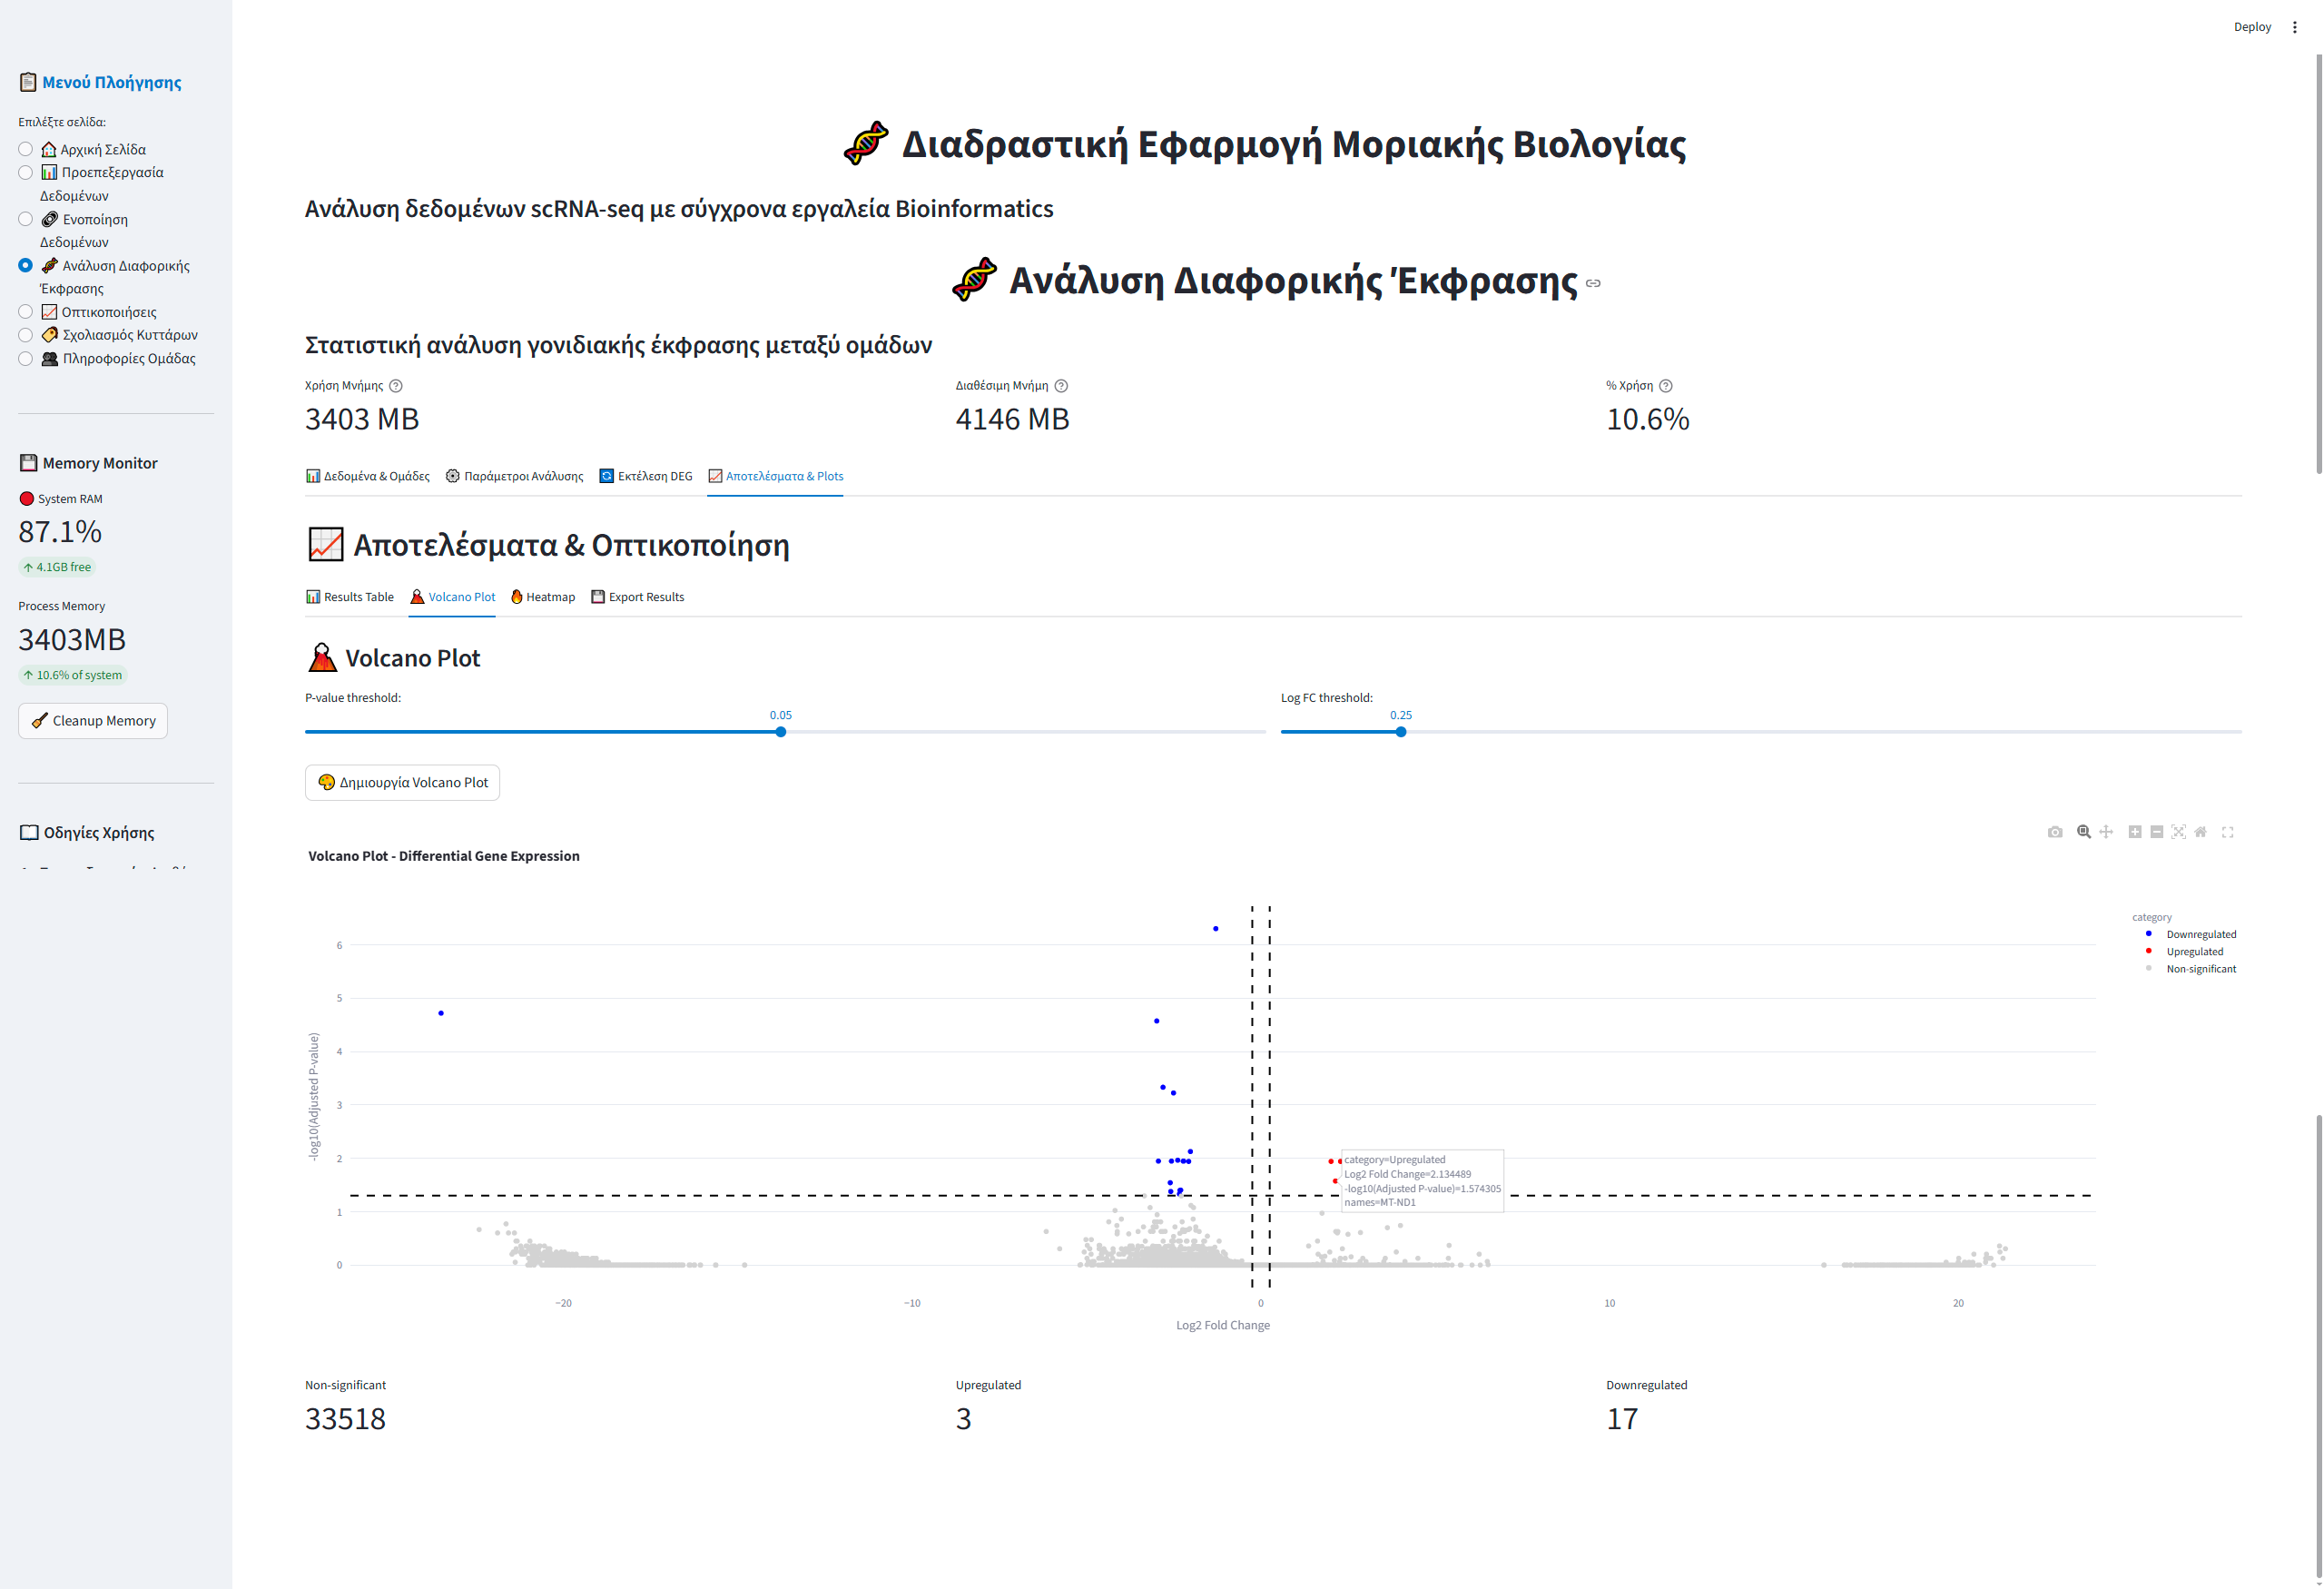
\includegraphics[width=1.0\linewidth]{volcano_plot.png}
        \caption{Volcano Plot}
    \end{subfigure}
    \hfill
    \begin{subfigure}{0.45\textwidth}
       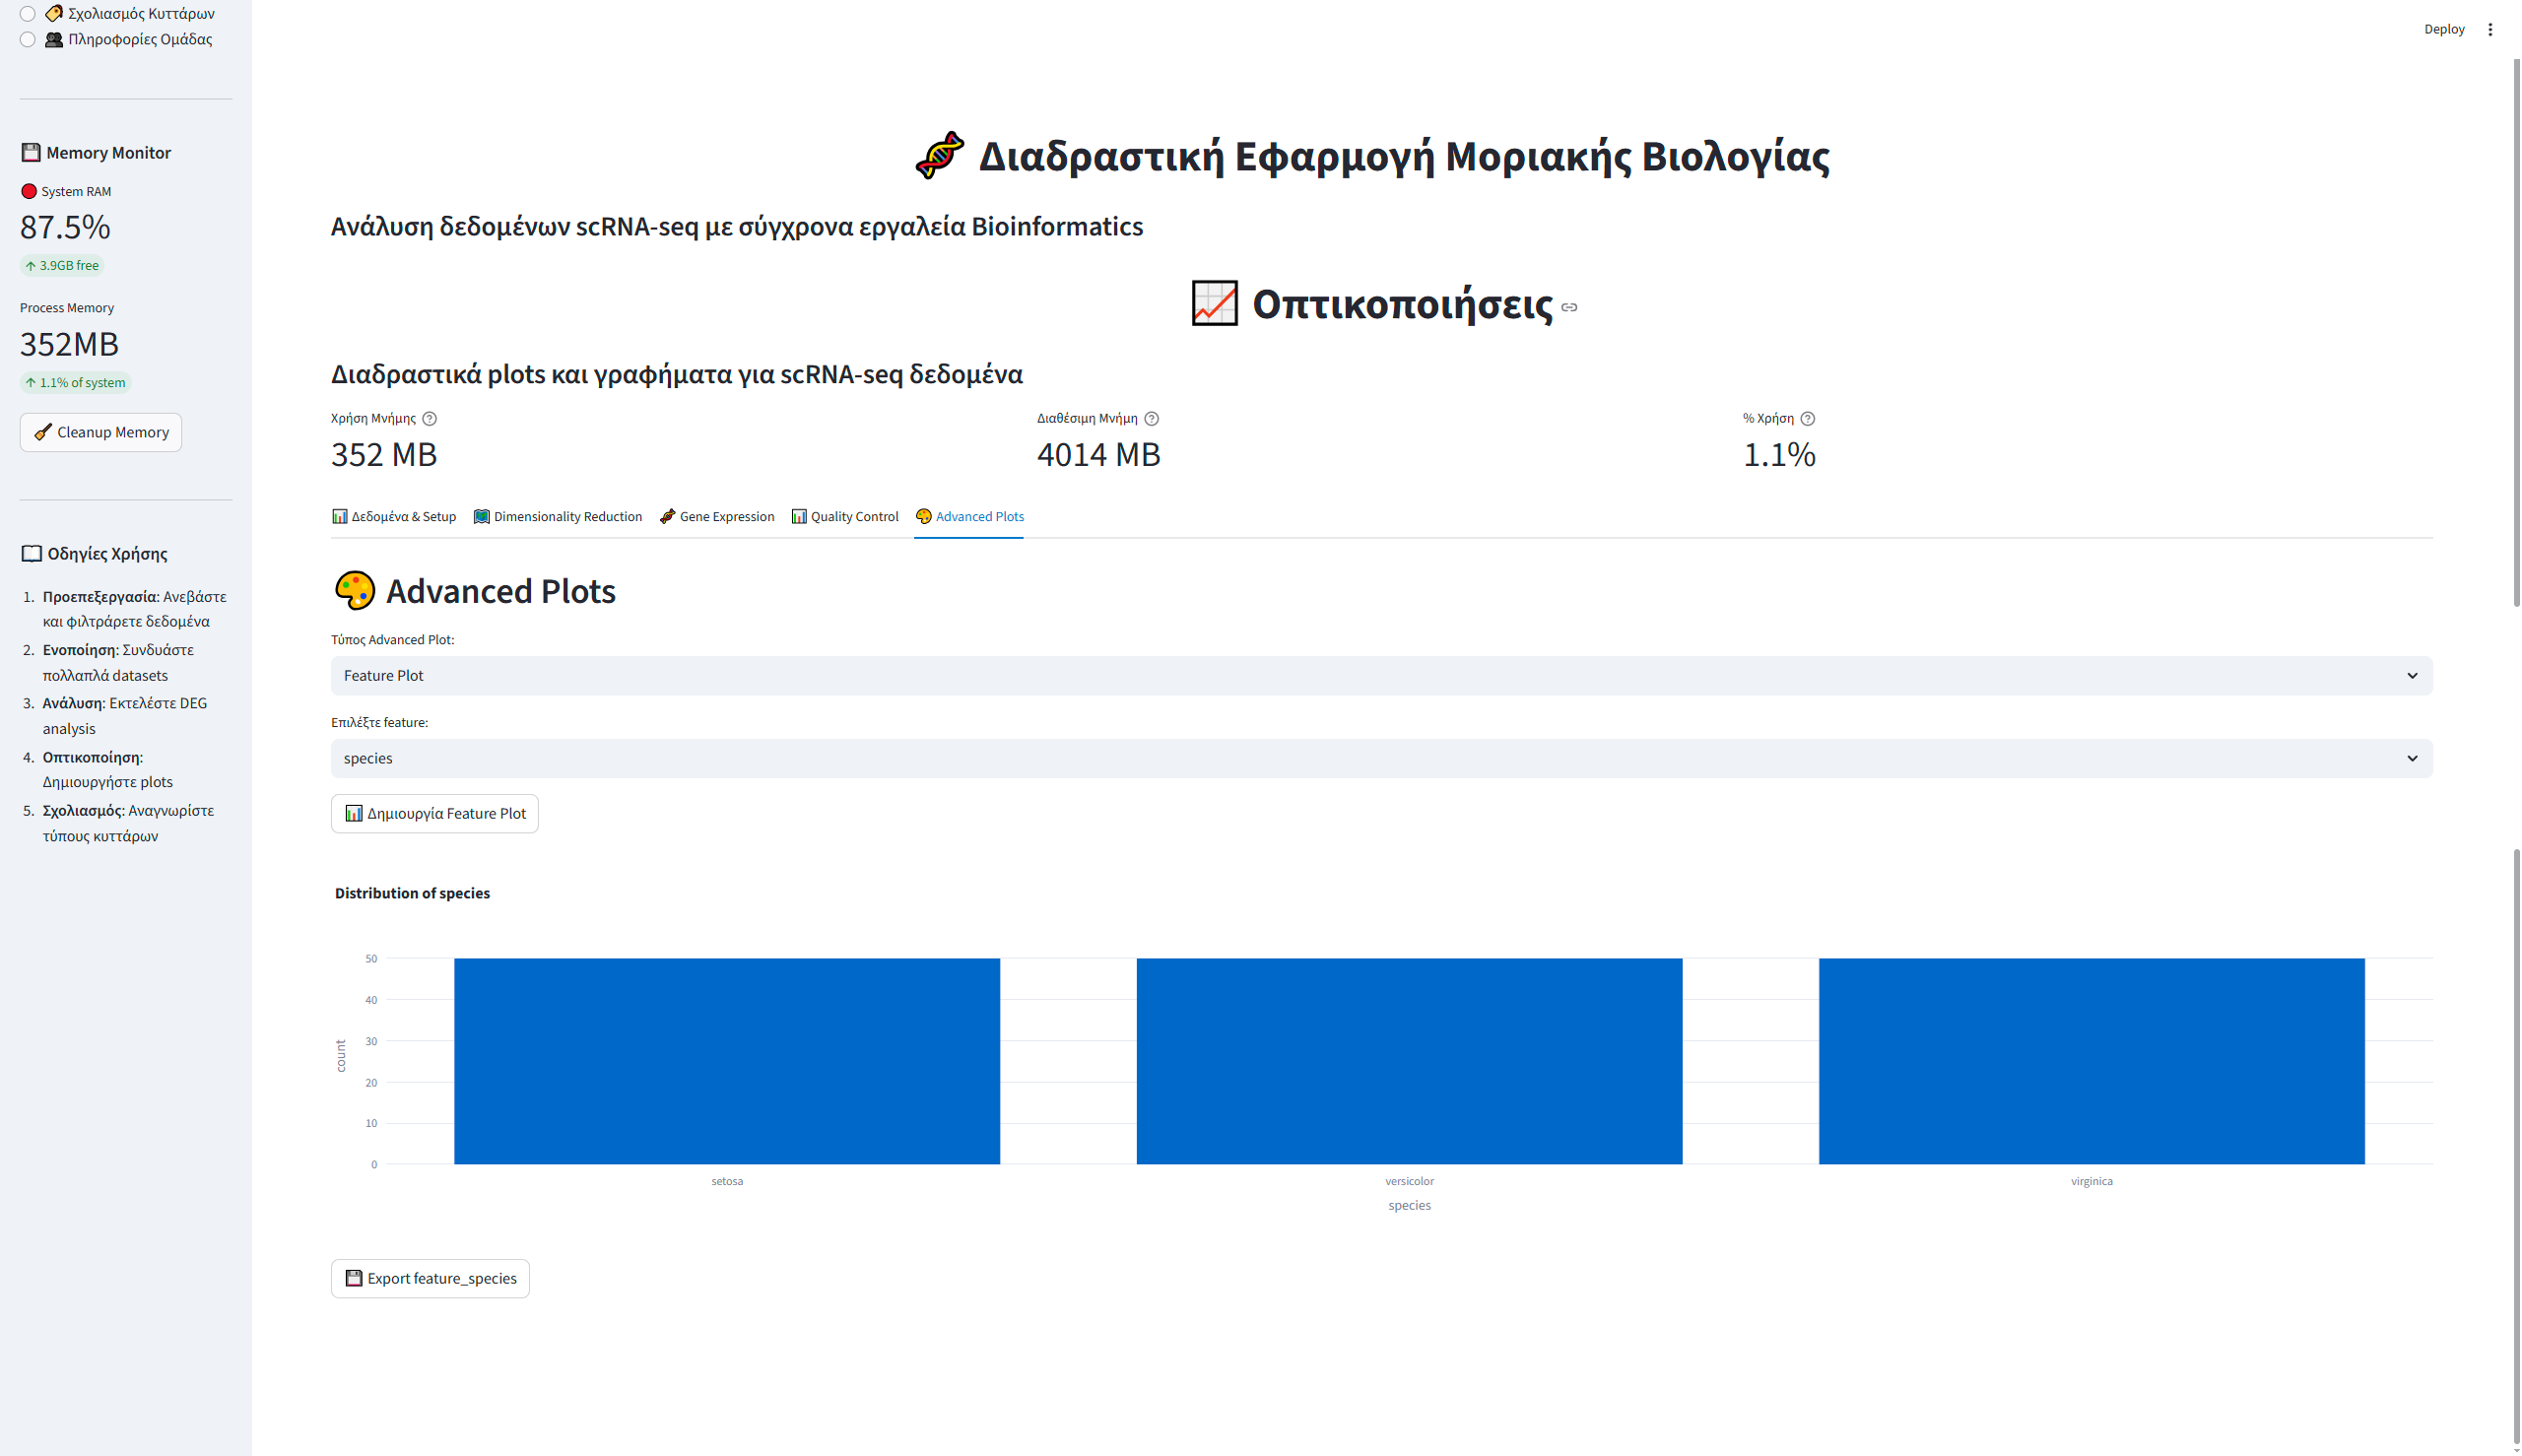
\includegraphics[width=1.0\linewidth]{extra_plots.png}
        \caption{Feature Κορυφαίων DEGs}
    \end{subfigure}
    \caption{Αποτελέσματα ανάλυσης διαφορικής έκφρασης}
    \label{fig:deg_results}
\end{figure}

\subsection{Αποτελέσματα Σχολιασμού Κυττάρων}

\begin{figure}[H]
    \centering
    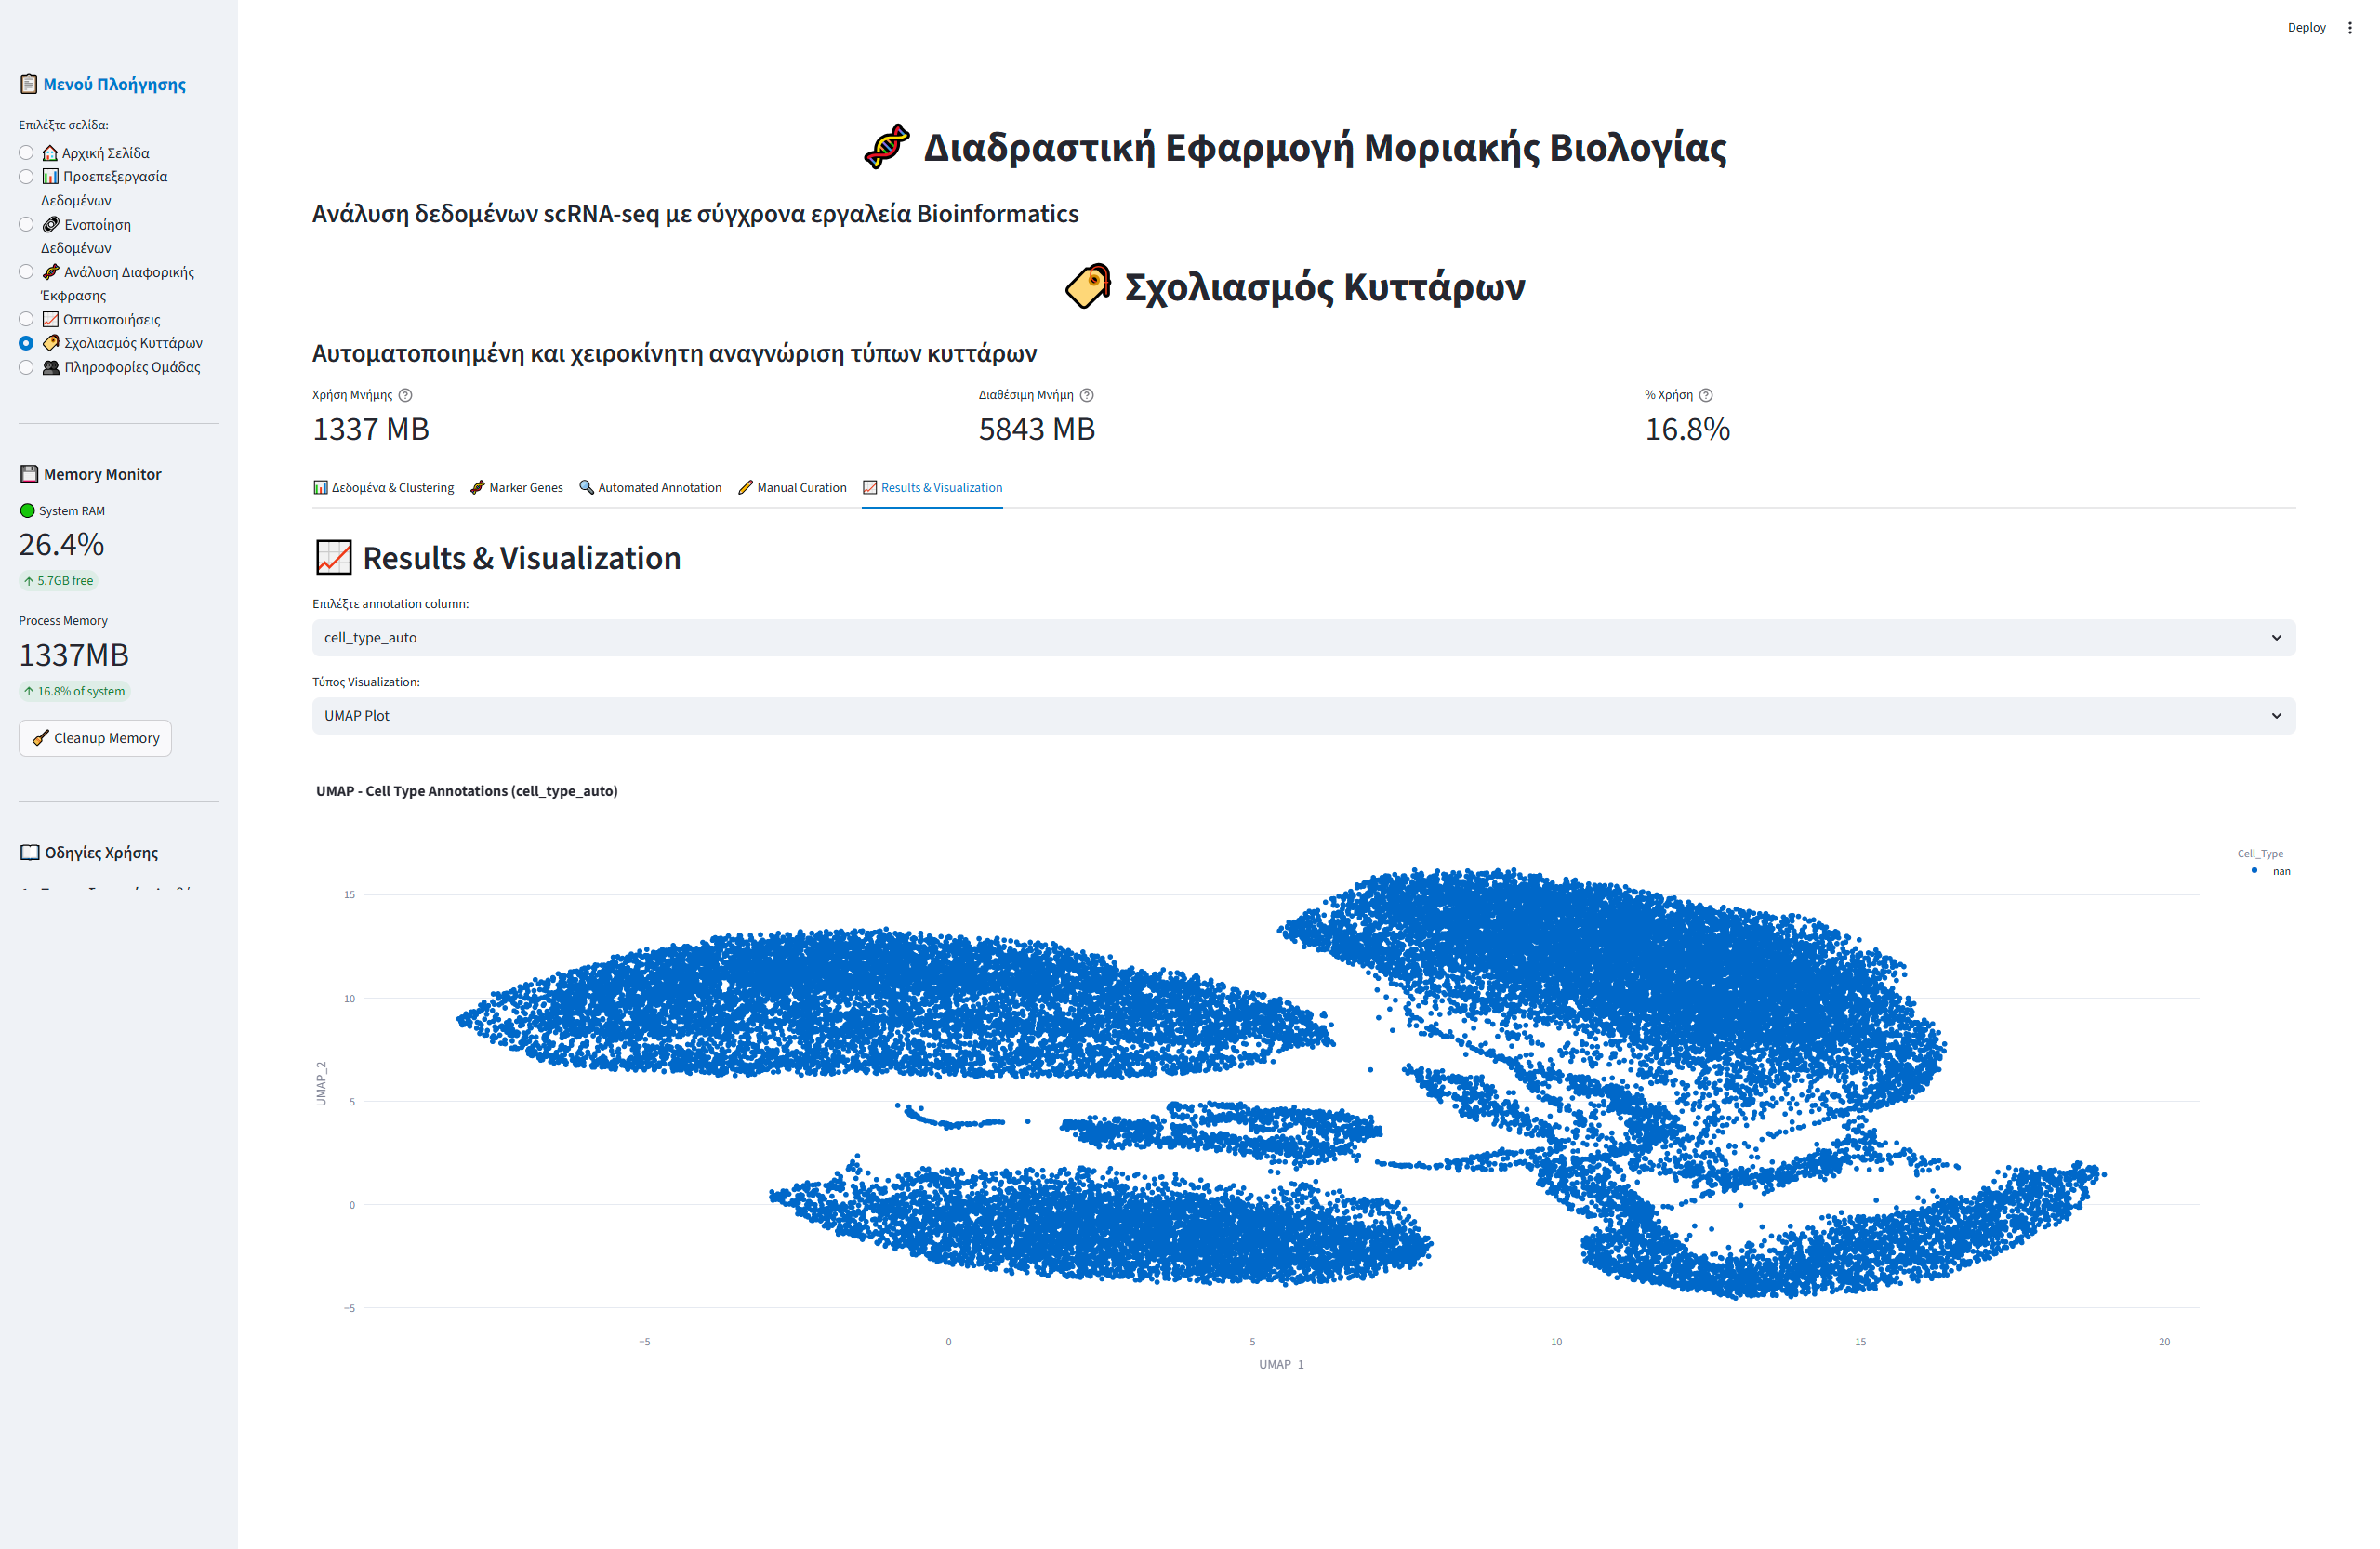
\includegraphics[width=1.0\linewidth]{annotation.png}
    \caption{Αποτελέσματα σχολιασμού τύπων κυττάρων επικαλυμμένα στο UMAP}
    \label{fig:cell_annotation}
\end{figure}

\section{Περιγραφή του Dockerization της Εφαρμογής}

\subsection{Αρχιτεκτονική Container}

Η εφαρμογή είναι πλήρως containerized με Docker, εξασφαλίζοντας αναπαραγώγιμες αναπτύξεις σε διαφορετικά περιβάλλοντα:

\begin{lstlisting}[language=Docker, caption={Υλοποίηση Dockerfile}]
FROM python:3.11-slim

# Εγκατάσταση εξαρτήσεων συστήματος για επιστημονικό υπολογισμό
RUN apt-get update && apt-get install -y \
    gcc g++ gfortran \
    libopenblas-dev liblapack-dev libhdf5-dev \
    pkg-config \
    && rm -rf /var/lib/apt/lists/*

# Εγκατάσταση εξαρτήσεων Python
COPY requirements.txt .
RUN pip install --no-cache-dir -r requirements.txt

# Αντιγραφή κώδικα εφαρμογής
COPY . /app
WORKDIR /app

# Έκθεση θύρας και εκτέλεση εφαρμογής
EXPOSE 8501
CMD ["streamlit", "run", "app.py", 
     "--server.port=8501", 
     "--server.address=0.0.0.0"]
\end{lstlisting}

\subsection{Διαμόρφωση Docker Compose}

Το αρχείο \texttt{docker-compose.yml} παρέχει ενορχήστρωση για ανάπτυξη παραγωγής:

\begin{lstlisting}[language=YAML, caption={Διαμόρφωση Docker Compose}]
version: '3.8'
services:
  molecular-biology-app:
    build: .
    ports:
      - "8501:8501"
    volumes:
      - ./data:/app/data
      - ./temp_files:/app/temp_files
    mem_limit: 8g
    mem_reservation: 4g
    cpus: '4.0'
    restart: unless-stopped
\end{lstlisting}

\subsection{Οφέλη Ανάπτυξης}

Η containerized προσέγγιση παρέχει διάφορα πλεονεκτήματα:

\begin{itemize}
    \item \textbf{Συνέπεια Περιβάλλοντος}: Ίδιο περιβάλλον εκτέλεσης σε ανάπτυξη, δοκιμές και παραγωγή
    \item \textbf{Διαχείριση Εξαρτήσεων}: Όλες οι βιβλιοθήκες επιστημονικού υπολογισμού συσκευασμένες μέσα στο container
    \item \textbf{Έλεγχος Πόρων}: Όρια μνήμης και CPU αποτρέπουν την εξάντληση πόρων
    \item \textbf{Κλιμακωσιμότητα}: Εύκολη οριζόντια κλιμάκωση για πολλαπλούς ταυτόχρονους χρήστες
    \item \textbf{Συντήρηση}: Απλοποιημένες ενημερώσεις και διαχείριση εκδόσεων
\end{itemize}

\begin{figure}[H]
    \centering
    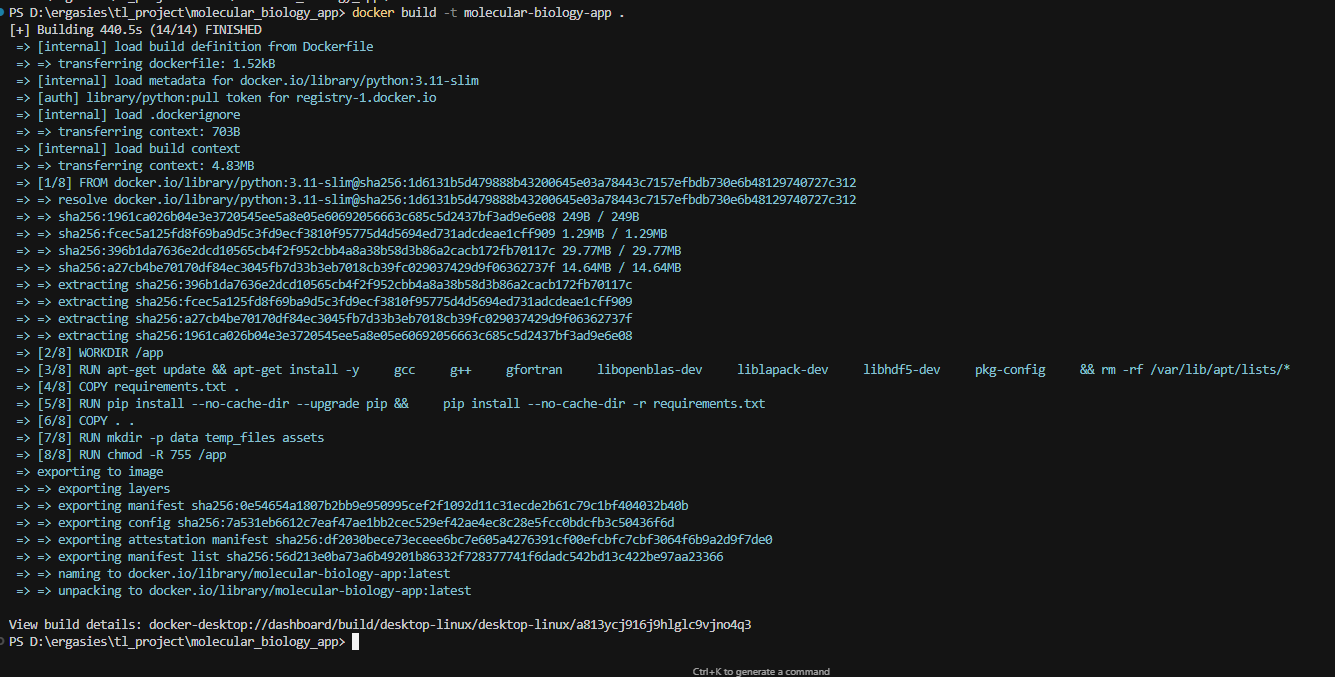
\includegraphics[width=1.0\linewidth]{docker_build.png}
    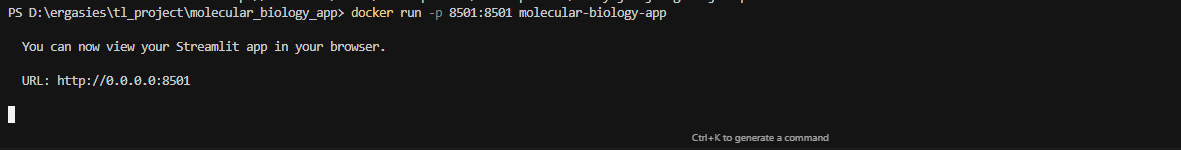
\includegraphics[width=1.0\linewidth]{docker_run.png}
    \caption{Διαδικασία ανάπτυξης Docker}
    \label{fig:docker_deployment}
\end{figure}

\subsection{Βελτιστοποίηση Απόδοσης στο Container}

Το container είναι βελτιστοποιημένο για φορτία εργασίας επιστημονικού υπολογισμού:

\begin{itemize}
    \item \textbf{Διαχείριση Μνήμης}: Όριο μνήμης 8GB με κράτηση 4GB
    \item \textbf{Κατανομή CPU}: 4 πυρήνες CPU για παράλληλη επεξεργασία
    \item \textbf{Επιστημονικές Βιβλιοθήκες}: Βελτιστοποιημένες βιβλιοθήκες BLAS/LAPACK για NumPy/SciPy
    \item \textbf{Έλεγχοι Υγείας}: Αυτοματοποιημένη παρακολούθηση υγείας για αναπτύξεις παραγωγής
\end{itemize}

\section{Συμπεράσματα}

Αυτή η εργασία παρουσιάζει μια ολοκληρωμένη, έτοιμη για παραγωγή πλατφόρμα για ανάλυση single-cell RNA sequencing που επιτυγχάνει επιτυχώς να αντιμετωπίσει τις βασικές προκλήσεις στις εφαρμογές βιοπληροφορικής:

\begin{enumerate}
    \item \textbf{Επίτευξη Κλιμακωσιμότητας}: Η εφαρμογή χειρίζεται αποδοτικά μεγάλα datasets μέσω προηγμένης διαχείρισης μνήμης και αλγορίθμων προσαρμοστικής κατάτμησης.
    
    \item \textbf{Επιστημονική Ακεραιότητα}: Όλες οι στατιστικές αναλύσεις διατηρούν επιστημονική αυστηρότητα χωρίς συμβιβασμούς στην απόδοση, εξασφαλίζοντας αξιόπιστα ερευνητικά αποτελέσματα.
    
    \item \textbf{Εμπειρία Χρήστη}: Η διαισθητική διεπαφή Streamlit κάνει την προηγμένη βιοπληροφορική προσβάσιμη σε ερευνητές χωρίς εκτεταμένη γνώση προγραμματισμού.
    
    \item \textbf{Ετοιμότητα για Παραγωγή}: Ολοκληρωμένος χειρισμός σφαλμάτων, παρακολούθηση σε πραγματικό χρόνο και containerized ανάπτυξη εξασφαλίζουν αξιοπιστία σε περιβάλλοντα παραγωγής.
    
    \item \textbf{Μοδουλαρικότητα και Επεκτασιμότητα}: Η μοδουλαρική αρχιτεκτονική διευκολύνει μελλοντικές βελτιώσεις και ενσωμάτωση νέων μεθόδων ανάλυσης.
\end{enumerate}

Μελλοντική εργασία θα επικεντρωθεί στην ενσωμάτωση επιπλέον μεθόδων ανάλυσης, την υλοποίηση επιτάχυνσης GPU για μεγαλύτερα datasets και την ανάπτυξη αυτοματοποιημένης βελτιστοποίησης pipeline βάσει χαρακτηριστικών dataset.

Ο πλήρης πηγαίος κώδικας και τεκμηρίωση είναι διαθέσιμα στο: \texttt{https://github.com/your-repo/molecular-biology-app}

\begin{figure}[H]
    \centering
    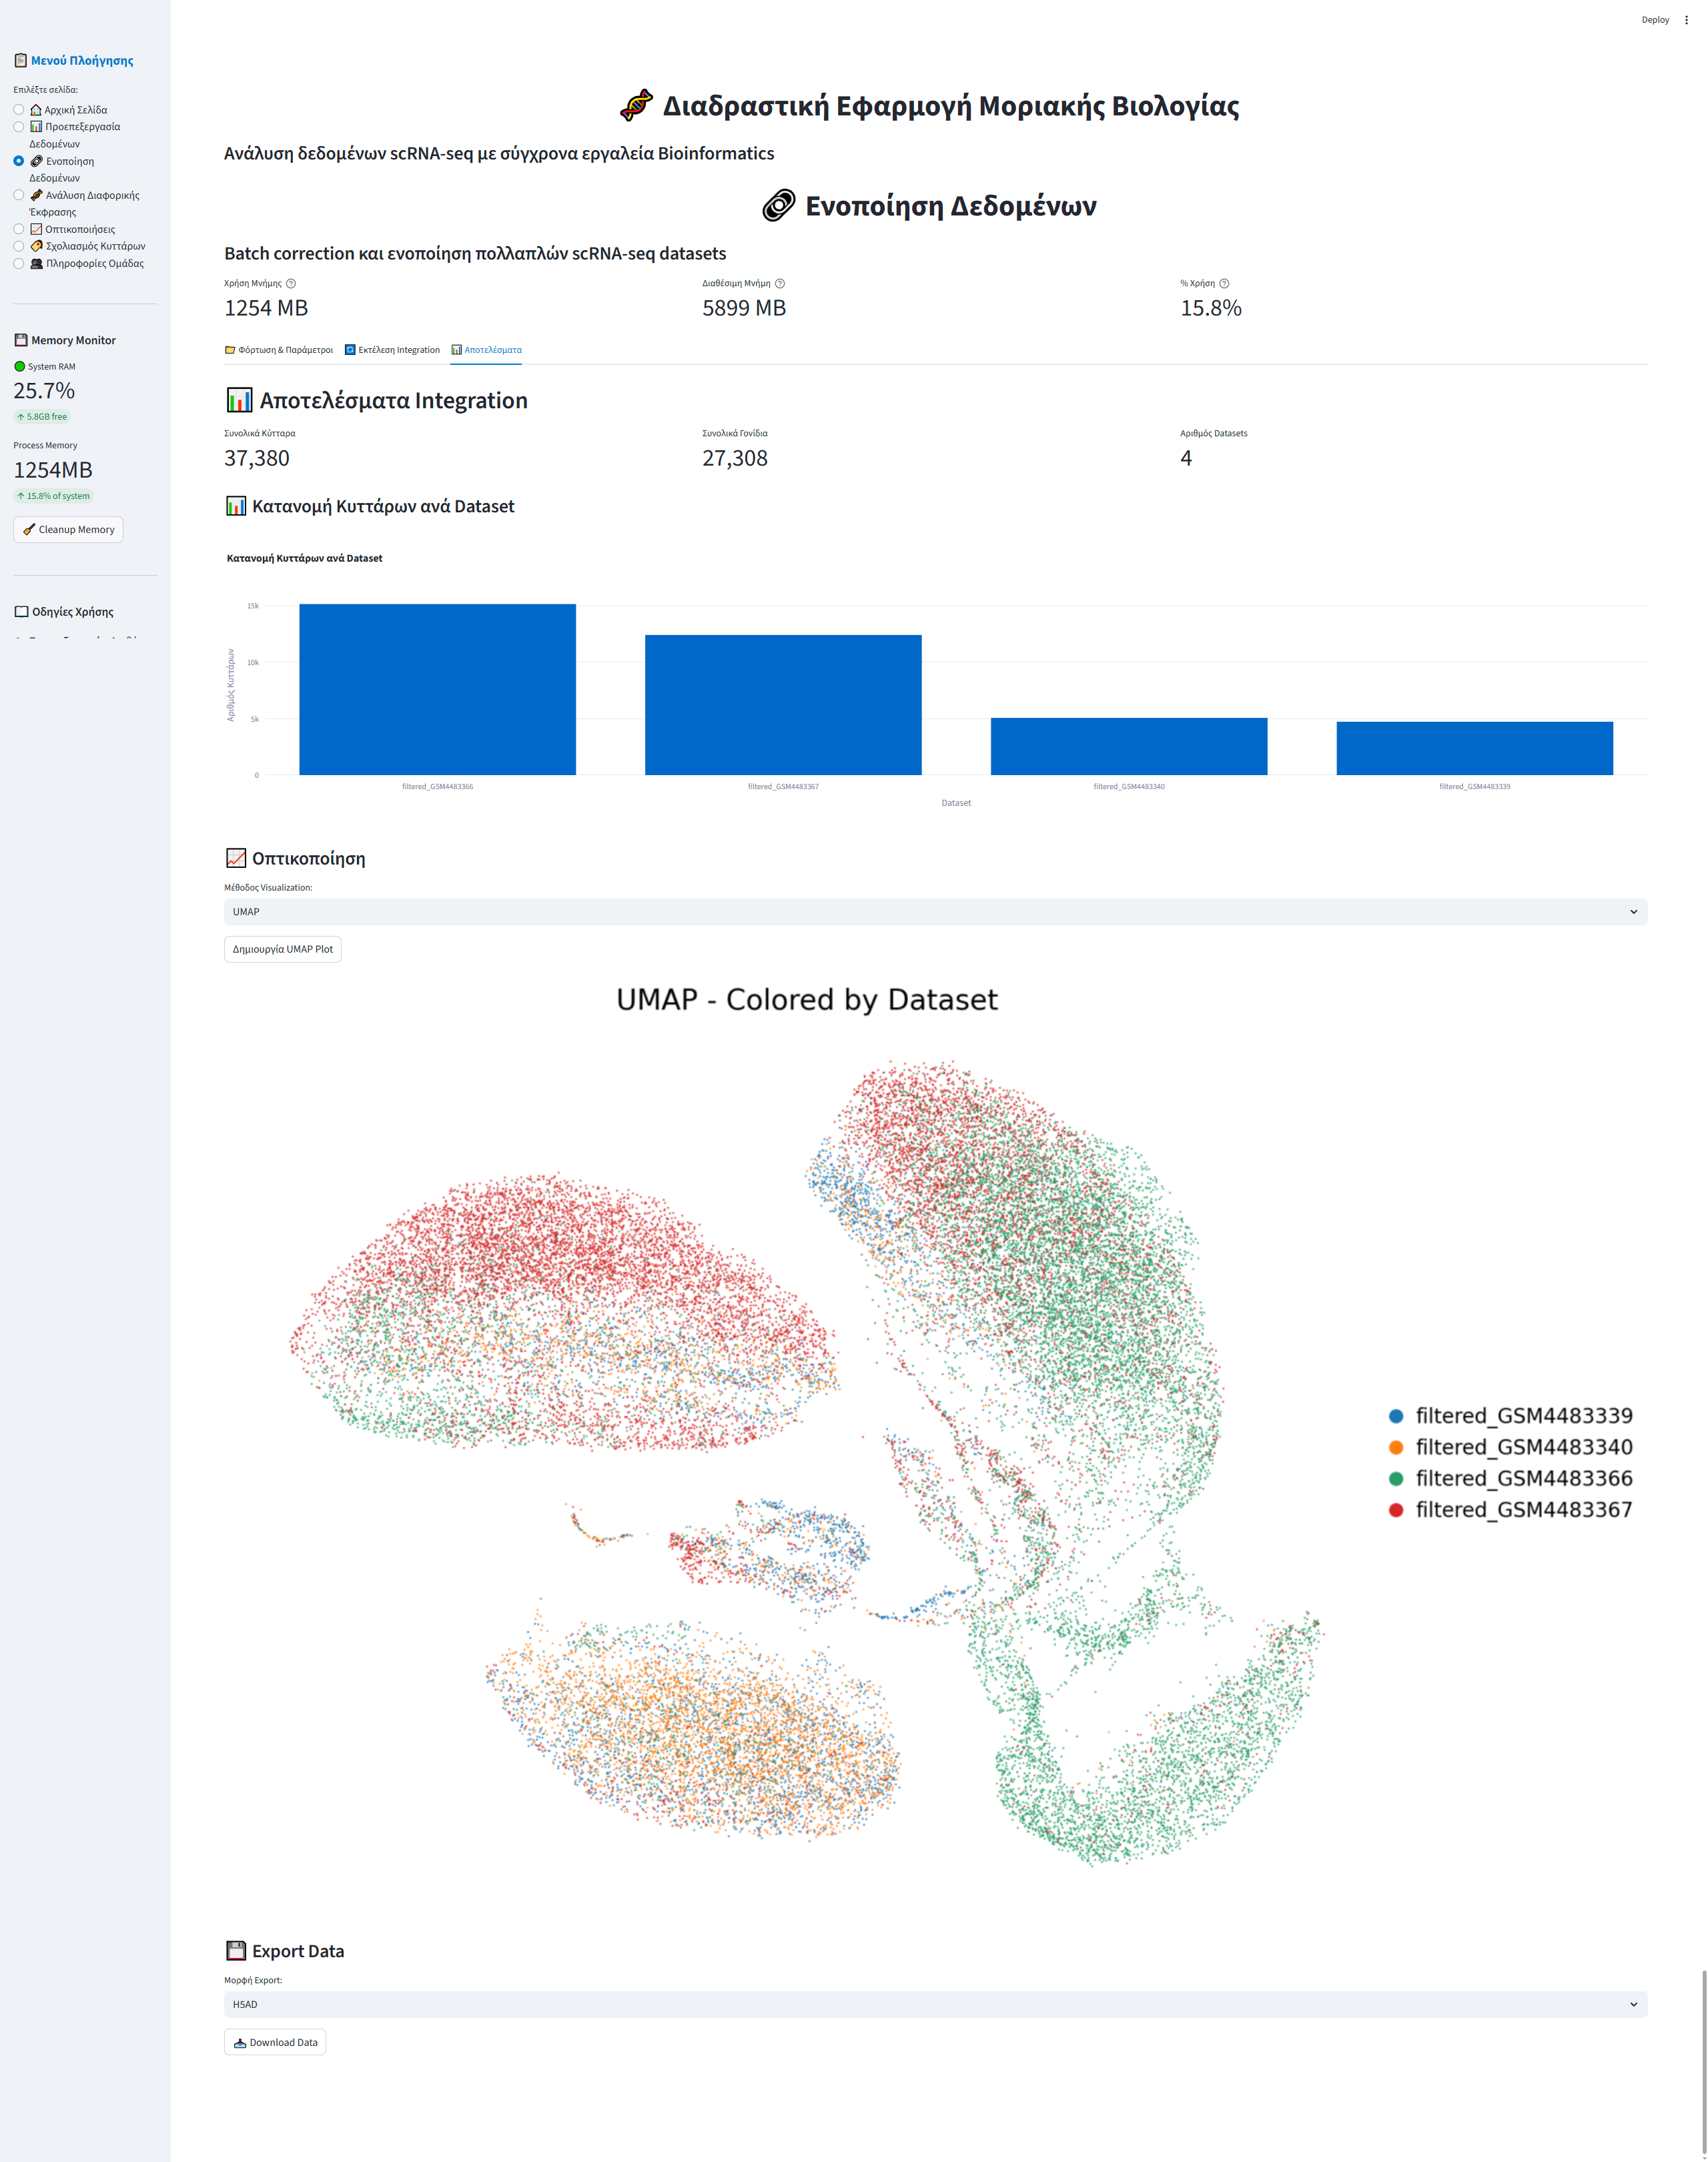
\includegraphics[width=1.0\linewidth]{graph_unified.png}
    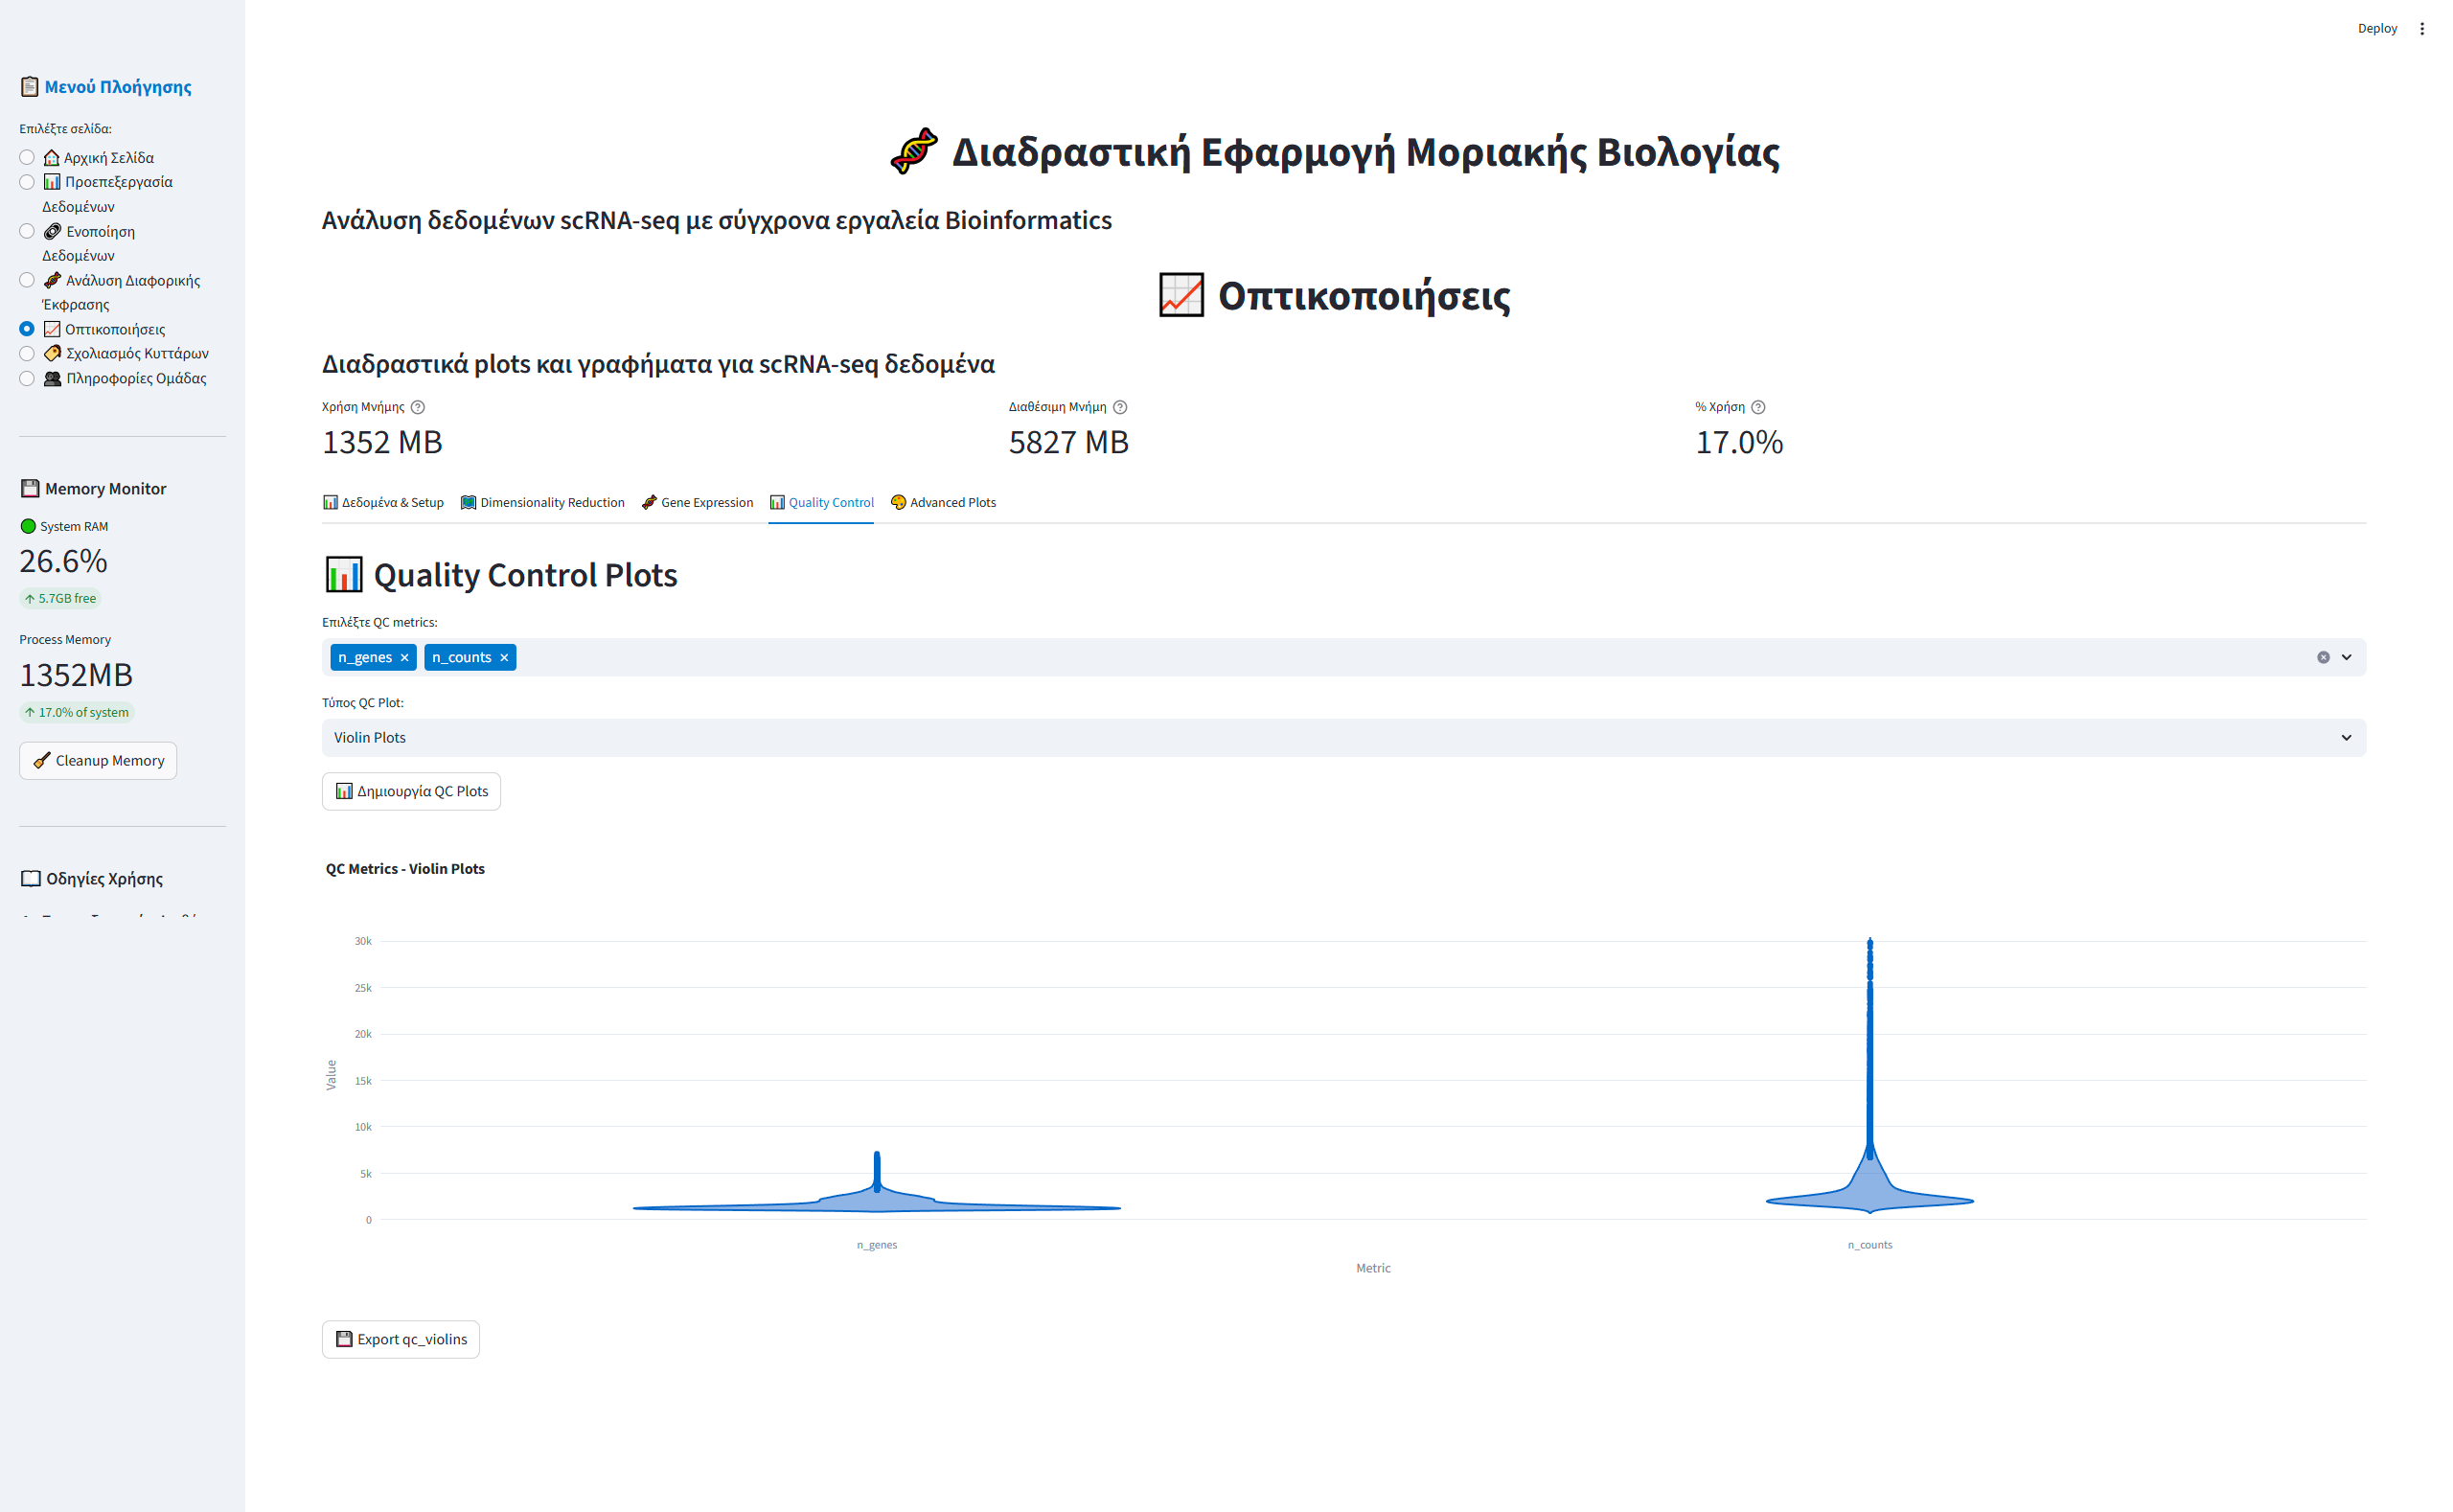
\includegraphics[width=1.0\linewidth]{violin_plots.png}
    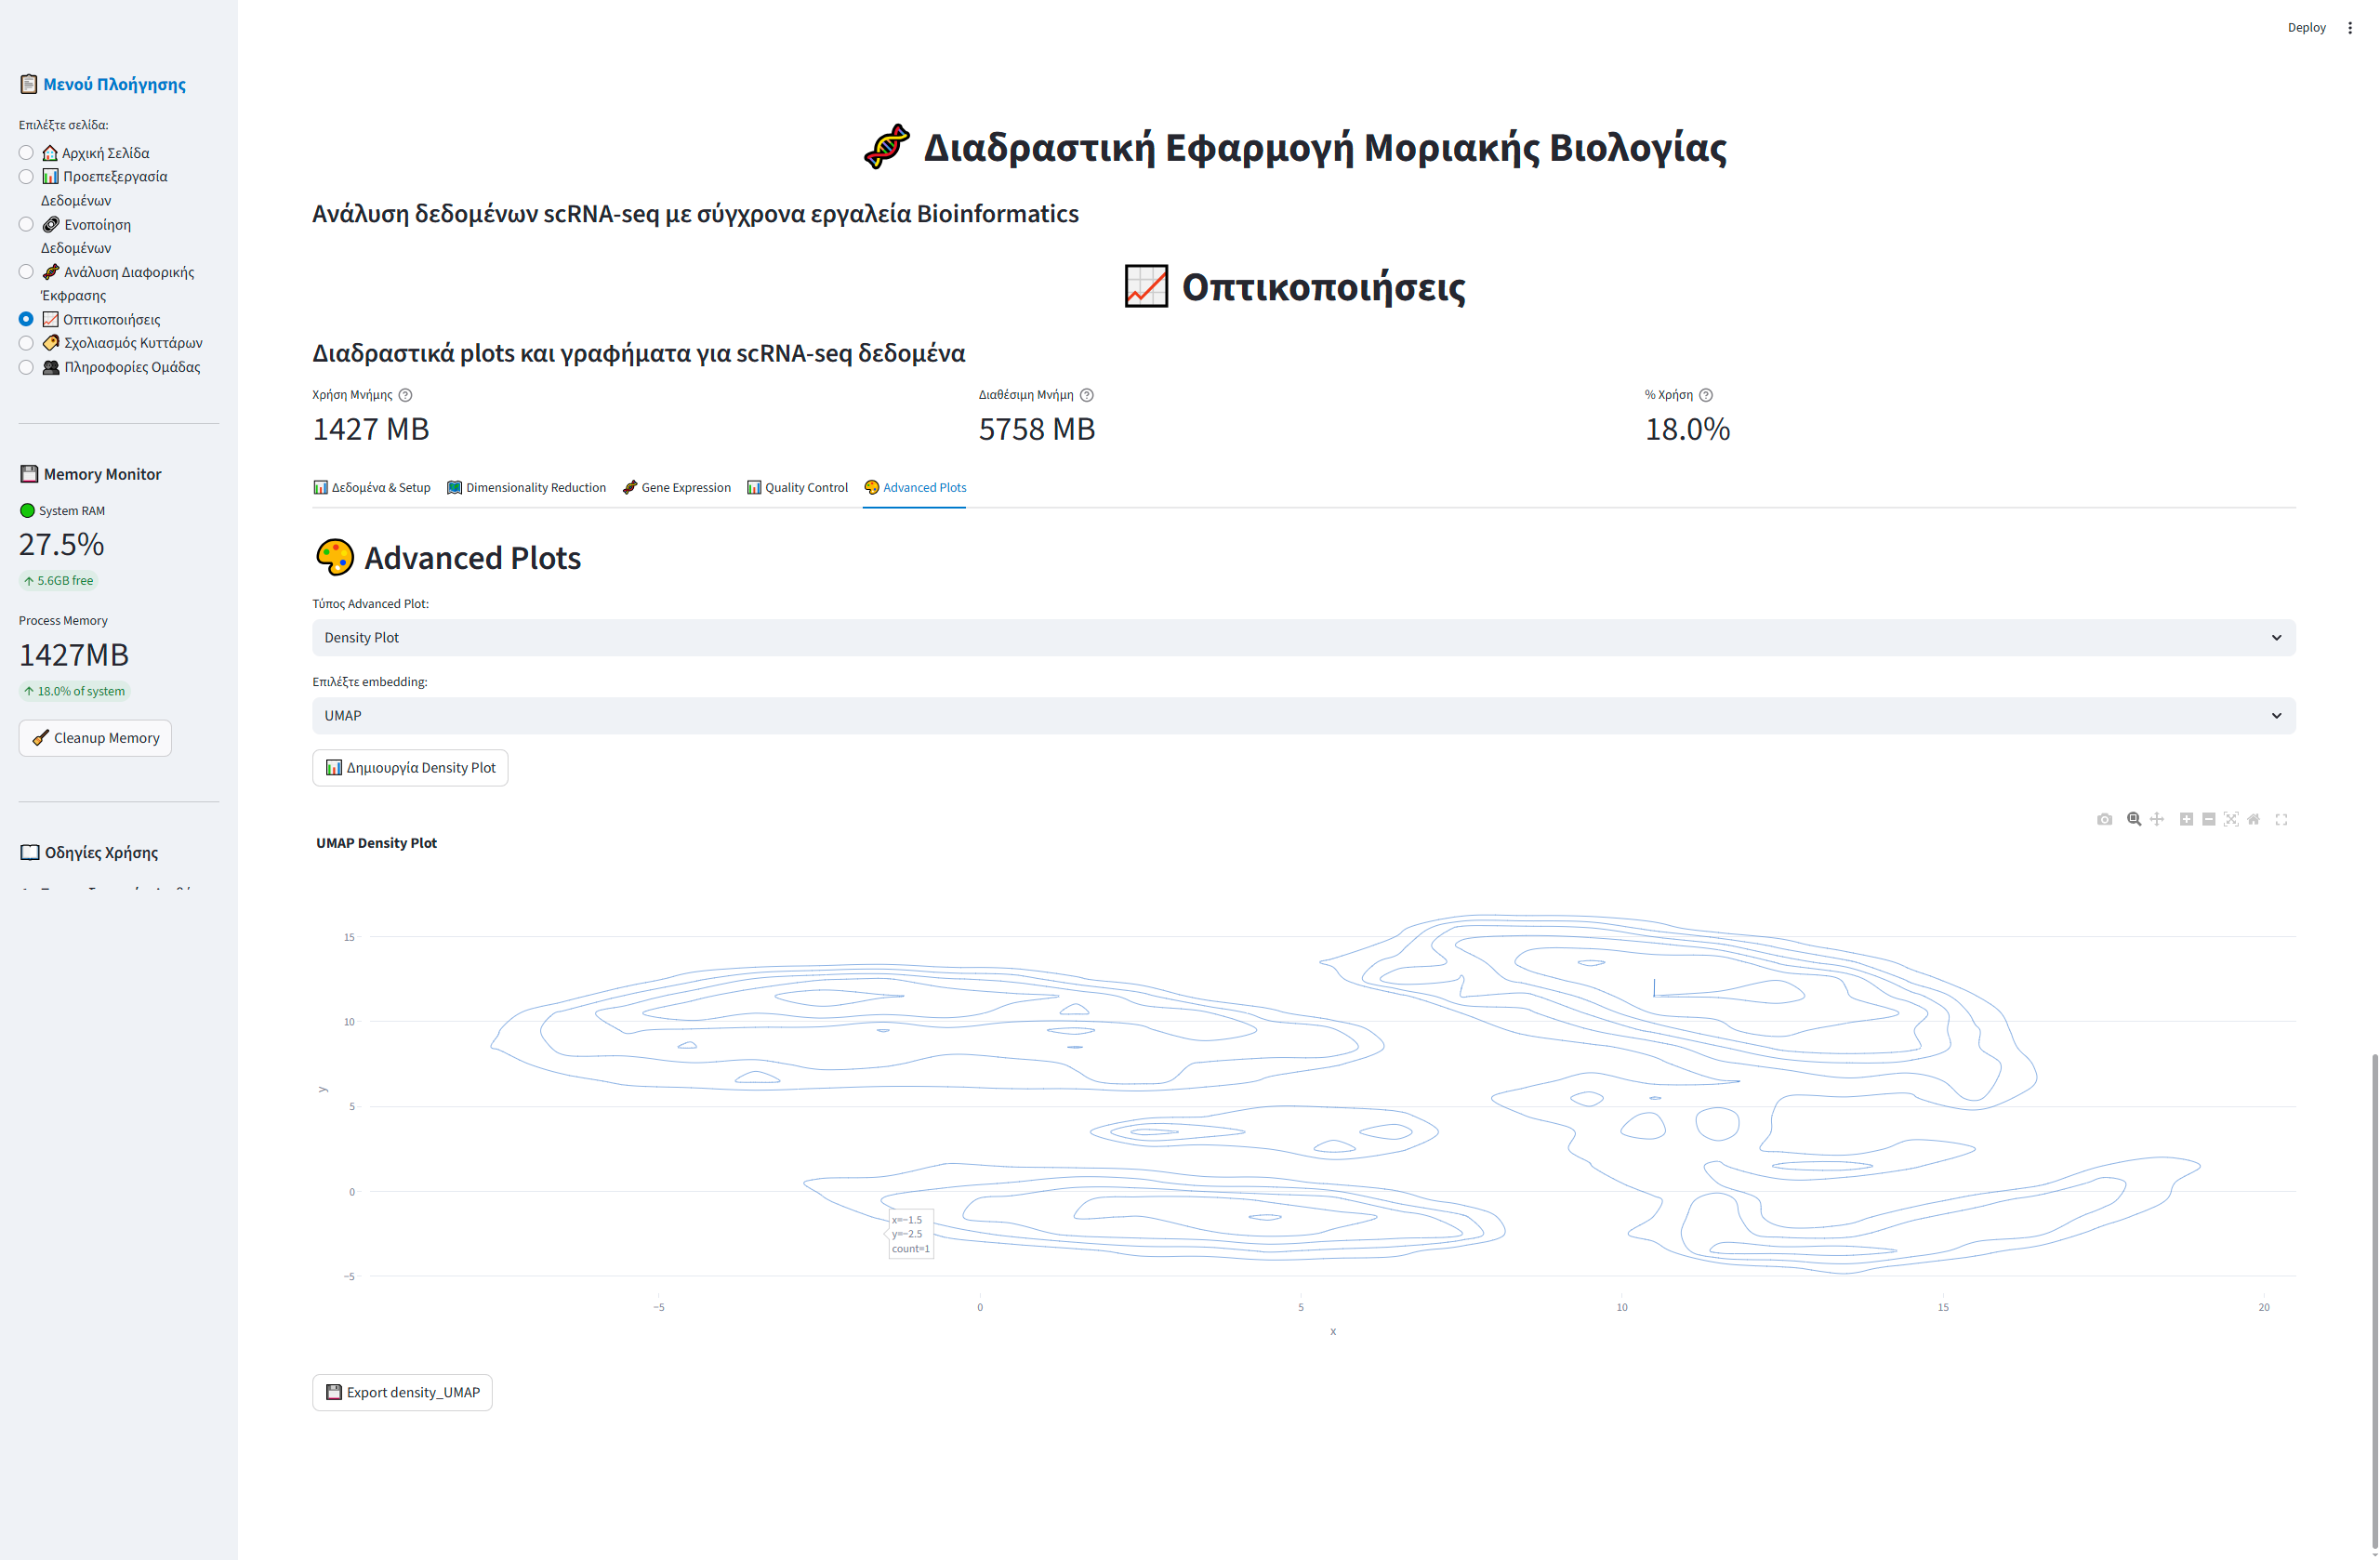
\includegraphics[width=1.0\linewidth]{density_plot.png}
    \caption{Πλήρης διεπαφή εφαρμογής που επιδεικνύει ενοποιημένη ροή εργασίας ανάλυσης}
    \label{fig:complete_interface}
\end{figure}

\begin{thebibliography}{9}
\bibitem{ref1} 
Tanay, A., \& Regev, A. (2017). Scaling single-cell genomics from phenomenology to mechanism. \textit{Nature}, 541(7637), 331-338.

\bibitem{ref2}
Wolf, F. A., Angerer, P., \& Theis, F. J. (2018). SCANPY: large-scale single-cell gene expression data analysis. \textit{Genome biology}, 19(1), 1-5.

\bibitem{ref3}
Korsunsky, I., Millard, N., Fan, J., Slowikowski, K., Zhang, F., Wei, K., ... \& Raychaudhuri, S. (2019). Fast, sensitive and accurate integration of single-cell data with Harmony. \textit{Nature methods}, 16(12), 1289-1296.

\end{thebibliography}

\end{document}
